%%%%%%%%%%%%%%%%%%%%%%%%%%%%%%%%%%%%%%%%%
% Vertical Line Title Page 
% LaTeX Template
% Version 1.0 (27/12/12)
%
% This template has been downloaded from:
% http://www.LaTeXTemplates.com
%
% Original author:
% Peter Wilson (herries.press@earthlink.net)
%
% License:
% CC BY-NC-SA 3.0 (http://creativecommons.org/licenses/by-nc-sa/3.0/)
% 
% Instructions for using this template:
% This title page compiles as is. If you wish to include this title page in 
% another document, you will need to copy everything before 
% \begin{document} into the preamble of your document. The title page is
% then included using \titleGM within your document.
%
%%%%%%%%%%%%%%%%%%%%%%%%%%%%%%%%%%%%%%%%%

%----------------------------------------------------------------------------------------
%	PACKAGES AND OTHER DOCUMENT CONFIGURATIONS
%----------------------------------------------------------------------------------------

\documentclass{book}

\newcommand*{\plogo}{\fbox{$\mathcal{PL}$}} % Generic publisher logo

%----------------------------------------------------------------------------------------
%	TITLE PAGE
%----------------------------------------------------------------------------------------

\newcommand*{\titleGM}{\begingroup % Create the command for including the title page in the document
\hbox{ % Horizontal box
\hspace*{0.2\textwidth} % Whitespace to the left of the title page
\rule{1pt}{\textheight} % Vertical line
\hspace*{0.05\textwidth} % Whitespace between the vertical line and title page text
\parbox[b]{0.75\textwidth}{ % Paragraph box which restricts text to less than the width of the page

{\noindent\Huge\bfseries The Simox Robotics Grasp Planner Library\\[0.5\baselineskip] \LaTeX ~Pandora@home}\\[2\baselineskip] % Title
{\large \textit{Programmers Manual}}\\[4\baselineskip] % Tagline or further description
{\Large \textsc{Kalogiannis Grigorios}} % Author name

\vspace{0.5\textheight} % Whitespace between the title block and the publisher
{\noindent Automation and Robotics Laboratory - Pandora@home \plogo}\\[\baselineskip] % Publisher and logo
}}
\endgroup}

%----------------------------------------------------------------------------------------
%	BLANK DOCUMENT
%----------------------------------------------------------------------------------------
\setcounter{secnumdepth}{5}
\usepackage{amsmath}
\usepackage{amssymb} % mathbb{}
\usepackage{algorithm}
\usepackage{algpseudocode}
\usepackage{bm}
\usepackage{subcaption} % subfigure environment 
\usepackage{algpseudocode}
\usepackage{pifont}
\usepackage{graphicx} % graphicspath
\usepackage{epstopdf} % for eps figures, must be after the graphicx usepackage
\usepackage{listings}
\usepackage{xcolor}
\usepackage{verbatim}
\usepackage{hyperref}
\usepackage{enumitem}
\usepackage{subfloat}
\usepackage{float}

\lstset { %
frame=single,
    breaklines=true,
    language=C++,
    backgroundcolor=\color{black!5}, % set backgroundcolor
    basicstyle=\footnotesize,% basic font setting
    basicstyle=\ttfamily,
                    keywordstyle=\color{blue}\ttfamily,
                    stringstyle=\color{red}\ttfamily,
                    commentstyle=\color{green}\ttfamily,
                    morecomment=[l][\color{magenta}]{\#}
}
\graphicspath{ {fig/} } % define default path for figures
\newcommand{\inr}[1]{\in \mathbb{R}^#1}

\usepackage{amsthm} % newtheorem
\newtheorem{definition}{Definition}[section]
\newtheorem*{remark}{Remark}
\newpage
\begin{document}

\pagestyle{empty} % Removes page numbers
\titleGM % This command includes the title page
\tableofcontents
\newpage

\chapter{Introduction}
\section{Robotic grasping}
Over the past decades, research in robotic grasping has flourished. Several algorithms have been developed for synthesizing robotic grasps in order to achieve stability,force-closure,task compatibility and other properties. Different approaches have been developed to meet these goals, and substantial improvements have been claimed. Thus,the availability of a large number of algorithms
for our purpose has made it difficult to choose, since their approaches and assumptions are different.
\section{Need of grasping planning tools}
\par
Automatic grasp planning is a difficult problem because of the huge number of possible hand configurations. Humans simplify the problem by choosing an appropriate prehensile posture appropriate for the object and task to be performed. By modeling an object as a set of shape primitives (spheres, cylinders, cones and boxes) grasping tools can use a set of rules to generate a set of grasp starting positions and pregrasp shapes. These generated data can then be tested on the object model. Several grasp planning tools offer also the functionality to evaluate and test the resulted grasp in order to present the best grasp to the user.
\section{Simox}
\subsection{Indroduction - What is Simox}
Simox is a lightweight platform independent C++ toolbox containing three libraries for 3D simulation of robot systems, sampling based motion planning and grasp planning. \par The Virtual Robot library is used to define complex robot systems which may cover multiple robots with many degrees of freedom. The robot structure and its visualization can be easily defined via XML files and environments with obstacles and objects to manipulate are supported. The libraries Grasp Studio and Saba use these definitions for planning grasps or collision-free motions.\par State-of-the-art implementations of sampling-based motion planning algorithms (e.g. Rapidly-exploring Random Trees) are served by the Saba library which was designed for efficient planning in high-dimensional configuration spaces. \par The library Grasp Studio offers possibilities to compute grasp quality scores for generic end-effector definitions (e.g. a humanoid hand). The implemented 6D wrench-space computations, offer the possibility to easily (and quickly) measure the quality of an applied grasp to an object. Furthermore, the implemented planners are able to generate grasp maps for given objects automatically.
\subsection{Components of Simox}
\subsubsection{VirtualRobot: The robot library}
The library VirtualRobot can be used to define complex robot systems, which may cover multiple robots with many degrees of freedom. The robot structure and its visualization can be easily defined via XML files and environments with obstacles and objects to manipulate are supported. Further, basic robot simulation components, as Jacobian computations and generic Inverse Kinematics (IK) solvers, are offered by the library. Beyond that, extended features like tools for analyzing the reachable workspace for robotic manipulators or contact determination for grasping are included. 
\subsubsection{Saba: The motion planning library}
With Saba, a library for planning collision-free motions is offered, which directly incorporates with the data provided by VirtualRobot. The algorithms cover state-of-the-art implementations of sampling-based motion planning approaches (e.g. Rapidly-exploring Random Trees) and interfaces that allow to conveniently implement own planners. Since Saba was designed for planning in high-dimensional configuration spaces, complex planning problems for robots with a high number of degrees of freedom (DoF) can be solved efficiently. 
\subsubsection{Grasp Studio: The grasp planning library}
The Grasp Studio library contains methods and tools used for measuring grasp qualities. Therefore an interface to the qhull library is provided to build convex hulls in 3D or 6D. The methods for measuring grasp qualities implement methods based on force-space related algorithms in 3D and a full implementation of 6D grasp wrench spaces is included. Grasping setups of simple end-effectors, multi-finger hands, multi-hand and multi-robot grasps can be evaluated by the Grasp Studio library. Grasp planners are implemented for building object specific grasp maps for given end-effectors. 
\chapter{Installation}
\section{Get Simox from a PPA}
You have the choice of either installing the simox package from our PPA or by compiling the sources (see below). The PPA/package currently is available only on Ubuntu distributions starting from Precise (12.04) up to and including Trusty (14.04).
\par
First, add the PPA to your list of repositories and then install the package via apt-get: 
\begin{lstlisting}
sudo add-apt-repository ppa:simox-dev/ppa
sudo apt-get update
sudo apt-get install simox
\end{lstlisting}
Keep in mind that this will only install simox without any special options enabled (e.g. bullet) and with Coin visualization support. 
\section{Get Simox from gitlab repository}
Retrieve the sources with: 
\begin{lstlisting}
git clone https://gitlab.com/Simox/simox.git
\end{lstlisting}
Or use a GUI-based GIT client to grab the sources from: 
\hyperref[simox gitlab]{'https://gitlab.com/Simox/simox.git'}
\section{Install dependencies}
You will need the following libraries installed on your system: 

\begin{description}
\item[$\bullet$ ] CMake $>$=2.8.3: A cross-platform, open-source build system.\hyperref[cmake]{http://www.cmake.org/} 
\item[$\bullet$ ] Boost $>$=1.42: Provides free peer-reviewed portable C++ source libraries.\hyperref[boost]{http://www.boost.org} 
\item[$\bullet$ ] Eigen $>$=3.0: A header-only C++ template library for linear algebra: matrices, vectors, and numerical solvers.\hyperref[Eigen]{http://eigen.tuxfamily.org} 
\end{description}
\subsection{Visualization / 3D Model support}
\newcounter{MyCounter}
\setcounter{MyCounter}{1}% initial value
\begin{enumerate}[label={\arabic{MyCounter}\addtocounter{MyCounter}{1}}]
\item Coin3D/Qt (recommended) For 3D visualization support Simox offers a plugin-like mechanism that can be extended in order to make your favorite 3D library usable. In the current version Coin3D/Qt support is already implemented allowing to handle Open Inventor file formats (.iv, .vrml) in combination with Qt-based GUIs. If you want to use this visualization supported you will additionally need the following libraries:
\begin{description}
\item[$\bullet$ ] Qt4 ($>$=4.6) or Qt5: Cross-platform application and UI framework.\newline 
\hyperref[qt]{http://qt-project.org/downloads} 
\item[$\bullet$ ] Coin3D ($>$=3.1.3): A high-level, retained-mode toolkit for effective 3D graphics development.\newline  \hyperref[coin3d]{https://bitbucket.org/Coin3D/coin} 
\item[$\bullet$ ] SoQt ($>$=1.5): A set of Qt GUI bindings for Coin3D library. \newline 
\hyperref[SoQt]{https://bitbucket.org/Coin3D/soqt} 
\end{description} 
\item OpenSceneGraph With OpenSceneGraph (OSG) a LGPL library can be used with Simox (instaed of the GPL-library Coin3D). OSG supports several file formats for 3D-model loading, e.g. 3dc, 3ds, flt, geo, iv, ive, lwo, md2, obj, osg, whereas some of them depend on external libraries which must be present on your system. Have a look at OSG's installation and plugin help pages. 
\begin{description}
\item[$\bullet$ ] Qt4 ($>$=4.6): Cross-platform application and UI framework. QT versions>=5 are not yet supported.\newline 
\hyperref[qt]{http://qt-project.org/downloads} 
\item[$\bullet$ ] OpenSceneGraph ($>$=3.0): A high performance 3D graphics toolkit.\newline  \hyperref[openscene]{http://www.openscenegraph.org} 
\end{description} 
\item No visualization support With this setup, visualization is disabled and hence, no collision detection can be performed. Nevertheless all operations which do not rely on 3d models, e.g. coordinate transformations, are still available. 
\end{enumerate}
\section{Linux}
Simox is tested on several Ubuntu platforms and there shouldn't be any problems with other distributions 
\begin{itemize}

\item[$\bullet$] In order to setup the dependencies, you could either 
\begin{itemize}
\item[$\bullet$] have a look at the package manager of your distribution (maybe the libs you will need are already installed) 
\item[$\bullet$] or you install them by hand, i.e. compile and install the sources.  
\item[$\bullet$] On an Ubuntu 14.04 system you can install the libraries (with coin support) the following way (on other systems the names of the libraries may differ slightly):
\end{itemize}
\item[$\bullet$] create a build directory, e.g \begin{lstlisting}
<path_to_your_simox_checkout>/build
\end{lstlisting}
\item[$\bullet$] Setup your environment variables (not needed if the dependencies were installed to the standard linux system paths, e.g. when the package management system was used) 
\begin{itemize}
\item[$\bullet$] \texttt{Eigen3\_DIR->Path to Eigen3}
\item[$\bullet$] \texttt{BOOST\_ROOT -> The Boost directory }
\item[$\bullet$] \texttt{Coin3D\_DIR -> The Coin3D library  }
\item[$\bullet$] \texttt{SoQt\_DIR -> the SoQt lib (Has to be compiled with the used Coin3D and Qt version)  }
\item[$\bullet$] \texttt{QT\_QMAKE\_EXECUTABLE -> The complete path to the qmake binary file. Usually located at } \begin{lstlisting}[language=bash]
<QtDir>/bin/qmake
\end{lstlisting}
\item[$\bullet$] \texttt{Simox\_DIR -> The path to your simox checkout }
\item[$\bullet$] \texttt{ An exemplary setup could look like this (\textbf{}). You can create a simox\_setpath.sh file and by calling source simox\_setpath.sh all exports are set in your shell environment. }

\item[$\bullet$] Create make files: 
\begin{itemize}
\item[$\bullet$] go to your build directory: cd a
\item[$\bullet$] call either ccmake .. or use the cmake-gui .. (see below for further information about cmake-gui) 
\item[$\bullet$] configure ('c' in ccmake) and generate make files ('g' in ccmake) 
\end{itemize}
\item[$\bullet$] Compile Simox 
\begin{itemize}
\item[$\bullet$] Now Simox with all examples can be compiled by typing 'make'. Optionally you can specify how many processes should be used for compiling (e.g. 'make -j4') 
\end{itemize}
\item[$\bullet$] IDE 
\begin{itemize}
\item[$\bullet$] You can use the make files within your favorite IDE, like Eclipse http://www.eclipse.org or QtCreator http://qt-project.org/doc/qt-5/topics-app-development.html (which can be used also for non-Qt projects) 
\end{itemize}
\end{itemize}
\end{itemize}
\begin{lstlisting}
sudo apt-get install build-essential libboost-all-dev libeigen3-dev libsoqt4-dev libcoin80-dev cmake cmake-gui libqt4-dev subversion
\end{lstlisting}
\section{Windows}
On Windows we recommend the Visual Studio series for development. Microsoft provides a free version, the Visual Studio Express Edition: http://www.microsoft.com/visualstudio/en-us/products/2010-editions/express. (todo: maybe the platform SDK or the Windows SDK have to installed with the VS express edition.) 
\subsection{IDE / Compiler}
\subsection{Download and install dependencies}
\begin{itemize}

\item[$\bullet$]CMake can be installed with the provided installer: http://www.cmake.org/cmake/resources/software.html
\item[$\bullet$]Boost binaries for windows can be found here: http://sourceforge.net/projects/boost/files/boost-binaries/ or you can build the libraries from source: http://www.boost.org 
\item[$\bullet$]Eigen is a header-only library that can be found here: http://eigen.tuxfamily.org. Eigen must not be configured or installed, it's enough to extract the files. 
\item[$\bullet$]Qt can be installed via the Qt SDK installer: http://qt-project.org/downloads. With Visual Studio versions above VS2010 you may need to compile Qt by hand. Use the latest src packege from here https://download.qt.io/official\_releases/qt/4.8/4.8.7/
\item[$\bullet$]Coin3D: Coin3D can be found at https://bitbucket.org/Coin3D/coin/wiki/Home The version 3.1.3 comes with a VS9 solution (located at build/msvc9/). For VS10+ you need to adapt some minor things (see below). Don't forget to set the COINDIR environment variable before building the install project.
\item[$\bullet$]SoQt: Can be found here: https://bitbucket.org/Coin3D/soqt Compile it (be sure the environment variable COINDIR is set properly). The current version (1.5.0) can be compiled with VS9 by using the solution file that is located in build/msvc9/soqt1.sln. 
\item[$\bullet$]
\end{itemize}If you run into troubles compiling Coin3D/SoQt have a look here: Coin3D\_Win\_Help
\subsection{Windows Environment Variables}
In order to allow smooth development we recommend to setup your windows environment variables according to your installation. Check, if the following entries are present at your system: 
\begin{itemize}

\item[$\bullet$]BOOSTDIR -> the boost directory  
\item[$\bullet$]COINDIR -> The Coin3D install directory   
\item[$\bullet$]QTDIR -> The Qt directory 
\item[$\bullet$]Simox\_DIR -> The directory where you checked out the simox source code.  
\item[$\bullet$]The \textbf{Path} variable should contain the following entries:  
\begin{itemize}
\item[$\bullet$]\textbf{\%QTDIR\%\textbackslash bin}
\item[$\bullet$]\textbf{\%COINDIR\%\textbackslash bin}  
\item[$\bullet$]\textbf{\%BOOSTDIR\%\textbackslash lib}
\end{itemize}
\end{itemize}
\section{Compile Simox}
You can use cmake, ccmake (on linux) or cmake-gui for setting up the compilation process. 
\begin{itemize}

\item[$\bullet$]Create a build directory (e.g. \$Simox\_DIR/build) and configure simox with cmake .. or by starting cmake-gui.  
\item[$\bullet$]Check, if all paths are found correctly. 
\item[$\bullet$]configure (until all entries are valid) and generate make/solution files 
\item[$\bullet$]Compile with make or open generated project files in your IDE (E.g. a cmake visual studio generator will create the following solution file \$Simox\_DIR/build/Simox.sln)  
\item[$\bullet$]The libraries will be located at BUILD\_DIR/lib and all binaries go to BUILD\_DIR/bin 
\item[$\bullet$]Debug / Release: On linux and mac you can switch between debug and release by setting the CMAKE\_BUILD\_TYPE variable either to Debug or to Release. When compiling with VisualStudio, you can select the build type within your IDE.\par   
\end{itemize}
Here is an exemplary setup with cmake-gui:\par
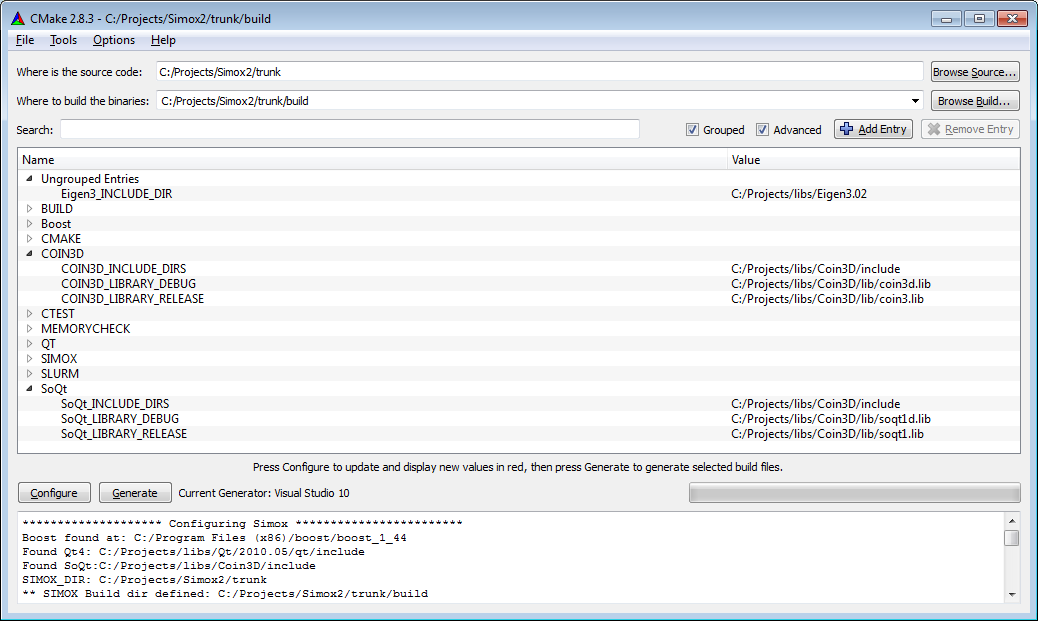
\includegraphics[width=\textwidth]{Simox_cmake_gui}
\section{Setup your own project}
\begin{itemize}
\item[$\bullet$] You can use the following CMake script in order to setup a project that relies on simox libraries. 
\item[$\bullet$] By calling FIND\_PACKAGE(Simox) the environment variable Simox\_DIR is queried in order to find the location of Simox. The simox version can be chosen by setting the environment variable Simox\_DIR to the build (e.g. /home/me/simox/build) or the install (e.g. /home/me/libraries/simox) directory. 
\begin{lstlisting}
    PROJECT ( myDemo )
    FIND_PACKAGE(Simox REQUIRED)
    IF(Simox_USE_COIN_VISUALIZATION)
      FILE(GLOB SRCS ${PROJECT_SOURCE_DIR}/myDemo.cpp ${PROJECT_SOURCE_DIR}/myWindow.cpp)
      FILE(GLOB INCS ${PROJECT_SOURCE_DIR}/myWindow.h)
      set(GUI_MOC_HDRS ${PROJECT_SOURCE_DIR}/myWindow.h)
      set(GUI_UIS ${PROJECT_SOURCE_DIR}/myWindow.ui)
      SimoxQtApplication(${PROJECT_NAME} "${SRCS}" "${INCS}" "${GUI_MOC_HDRS}" "${GUI_UIS}")
    ENDIF()
\end{lstlisting}
\end{itemize}

\chapter{Inside Simox}
\section{Inside the VirtualRobot library}
With the Virtual Robot library robots and environments can be specified and accessed via XML definitions. The structure of a robot is given by its joints (called RobotNodes) which are defined via Denavit-Hartenberg conventions or an easy-to-use "Translation+Rotation" scheme. The robot specification holds further information as name, joint limits, sensors, visualization and collision models. For convenient access kinematic chains and collections of collision models can be additionally defined. An instance of such a robot definition can be visualized by a viewer to show the current state of a robot. Furthermore, environments, obstacles and objects to manipulate can be defined and visualized. Thus it is possible to construct complex scenes used for simulation or planning and to store and load such scene definitions to/from XML files. The main features of the library are:
\begin{description}
  \item[$\bullet$ ]The library defines an interface for collision checking, allowing to exchange the collision checker used for determining distances or collisions. Currently the PQP collision checker is used due to its fast and robust implementation.
  \item[$\bullet$ ] A generic computation of Jacobains and its Pseudoinverse are offered for arbitrary kinematic chains.
   \item[$\bullet$ ] A generic IK solver, utilizing randomized approaches, is implemented for solving the IK for redundant kinematic chains.
   \item[$\bullet$ ]Reachability distributions are supported, in order to precompute the 6D reachability of a kinematic structure (e.g. an arm) and to quickly decide whether a pose in workspace is reachable or not.
   \item[$\bullet$ ]A generic definition of end effectors allows to realize complex hands (e.g. humanoid hands can be defined). End effectors can be opened/closed and contact information can be retrieved e.g. for grasp scoring.
   \item[$\bullet$ ]It is possible to store and load object-related grasping information for a given end-effector, which directly can be used within the IK solvers.
   \item[$\bullet$ ]Multithreading is supported, e.g. multiple instances of the collsiion checker can be used to parallelize collision queries. 
\end{description}

\subsection{Build a robot/environment model}
Robot models are defined via XML files, where the kinematic structure as well as additional information (e.g. visualizations, joint definitions or physics information) is stored. A robot consists of so-called Robot Nodes, which hold joint definitions and visualization data. After loading, these data structures can be accessed through the VirtualRobot library.\par In the following examples we start with a simple robot system in order to show how the XML definitions are structured. Later more complex examples are given, where you can see how advanced robot definitions can be created. \par

\subsubsection{Minimal Example}
\par
This minimal example shows how to define a robot. The file can be found in the doc/tutorial folder of the simox source tree. It can be loaded with VirtualRobot's RobotViewer example (located at VirtualRobot/examples/RobotViewer). 
\par
\begin{lstlisting}
<Robot Type="DemoRobot" RootNode="root">

   <RobotNode name="root">
   </RobotNode>

</Robot>
\end{lstlisting}
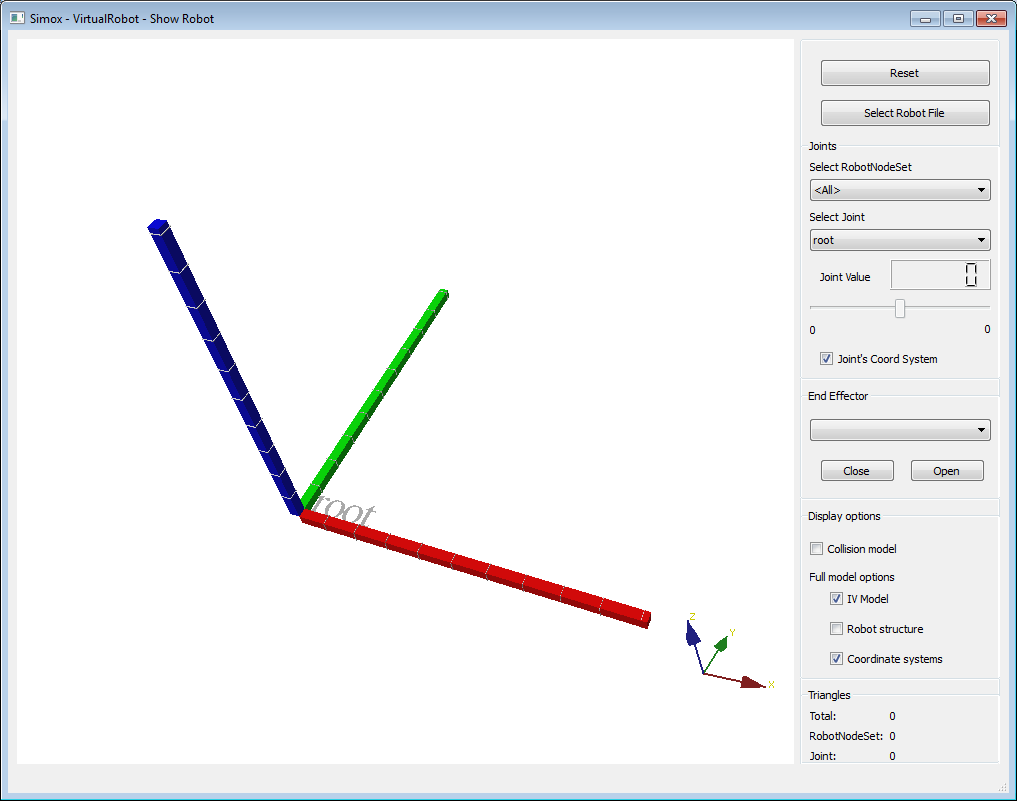
\includegraphics[width=\textwidth]{Tutorial1}
\par
\subsubsection{Visualizations}
\par
Now we add a visualization. In the following example, the Coin3D/Qt visualization support is used, indicated by the type="Inventor" attribute of the visualization's File tag (in case OpenSceneGraph is used for 3D-model importing and visualization, the attribute would be type="osg"). The location of the joint.iv file is given relatively to the location of the XML file, so that the directory iv is searched for the file joint.iv. 
\begin{lstlisting}
<Robot Type="DemoRobot" RootNode="root">

   <RobotNode name="root">
       <Visualization>
           <File type="Inventor">iv/joint.iv</File>
    </Visualization>
   </RobotNode>

</Robot>
\end{lstlisting}
\par
The joint.iv file defines a cylinder in the OpenInventor format. As specified in OpenInventor, the cylinder is aligned with the y axis and it is 500 mm long. In order to set one side of the cylinder to the (local) origin, the object is moved by 250 mm. 
\par
\begin{lstlisting}
#Inventor V2.0 ascii
Separator {
   Translation {
       translation 0 250 0
   }
   Cylinder {
       radius 40
       height 500
       parts (SIDES | TOP | BOTTOM)
   }
}
\end{lstlisting}
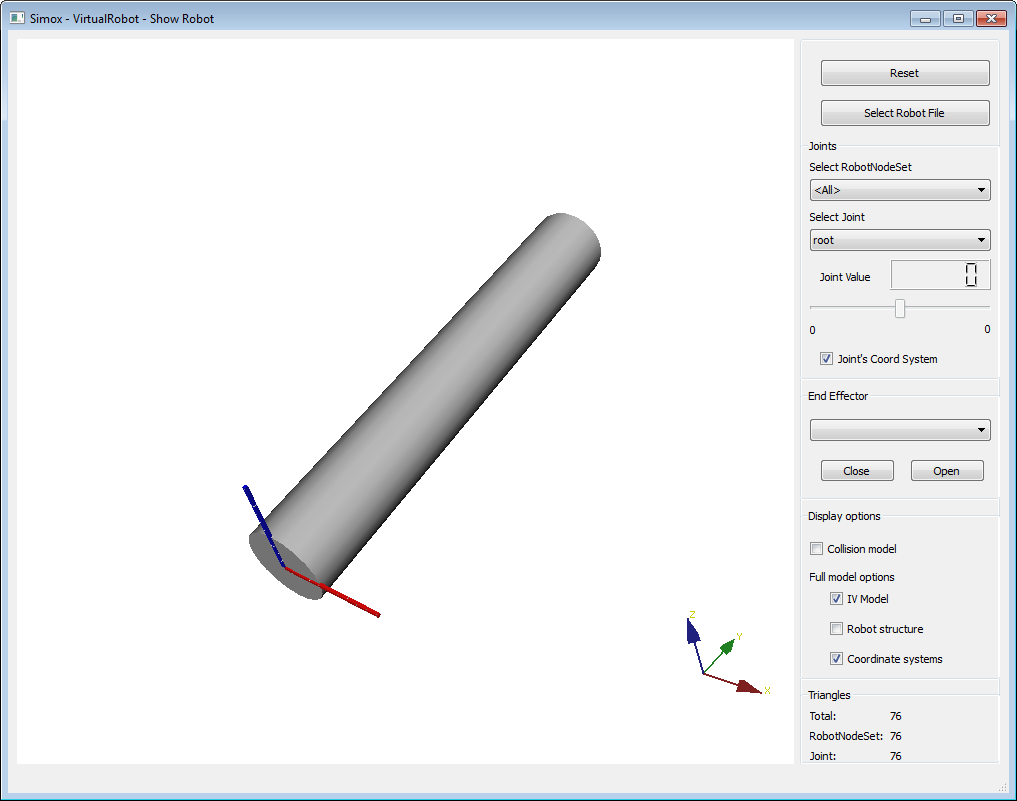
\includegraphics[width=\textwidth]{Tutorial2}
\par
\subsubsection{Joints}
\par
In this example the robot gets a movable joint. The Joint type is specified with the revolute attribute and the rotation axis. The Transform tag specifies a fixed transformation that is applied before the joint. Hence, a RobotNode may imply two transformations:
\begin{description}
   \item[$\bullet$] Transform This fixed transformation is applied to the parent's global pose.
 \item[$\bullet$]Joint: This transformation depends on the joint value and the resulting pose specifies the location where the visualization is linked to. This final pose of the RobotNode is noted as GlobalPose in Simox. This is the starting point for computing the coordinate systems of all children. 
\end{description}
\par
\begin{lstlisting}
<Robot Type="DemoRobot" RootNode="root">

  <RobotNode name="root">
    <Child name="joint 1"/>
  </RobotNode>

  <RobotNode name="joint 1">
    <Transform>
      <Translation x="0" y="500" z="0"/>
    </Transform>
    <Joint type="revolute">
      <Axis x="0" y="0" z="1"/>
    </Joint>
    <Visualization>
      <File type="Inventor">iv/joint.iv</File>
    </Visualization>
  </RobotNode>

</Robot>
\end{lstlisting}

\begin{figure}[H]
	\centering
	\begin{minipage} {.45\linewidth}
	  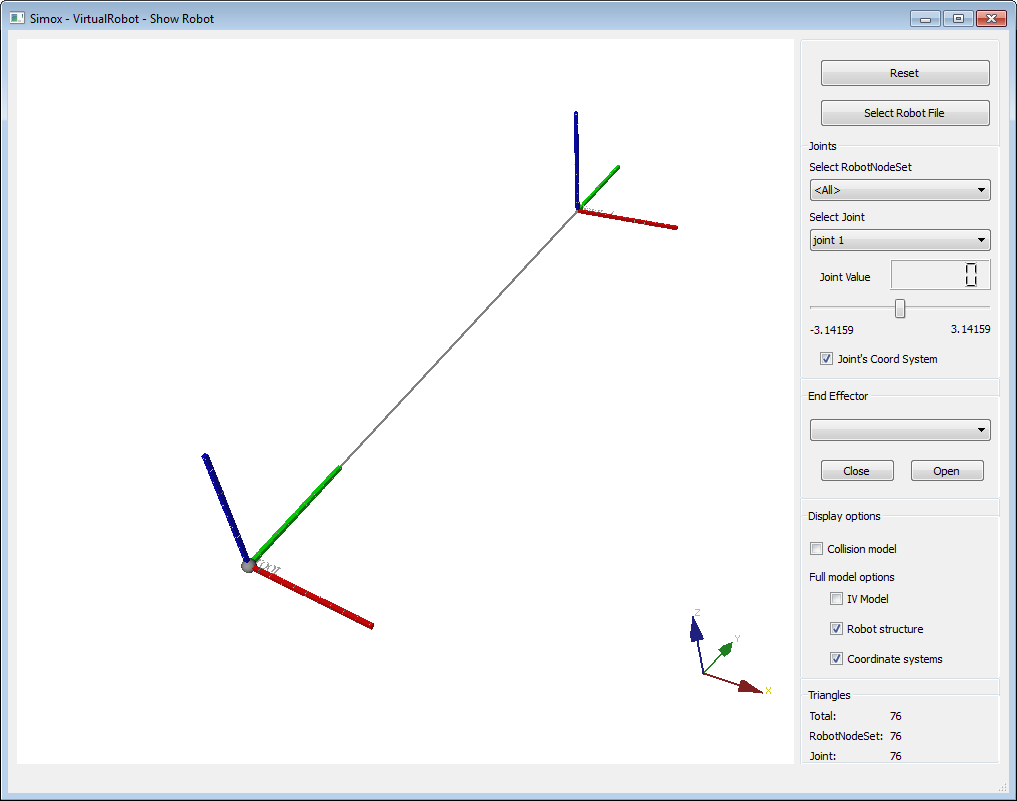
\includegraphics[width=\linewidth]{Tutorial3a}
	\end{minipage}
	%\hspace{.05\linewidth}
	\begin{minipage} {.45\linewidth}
	  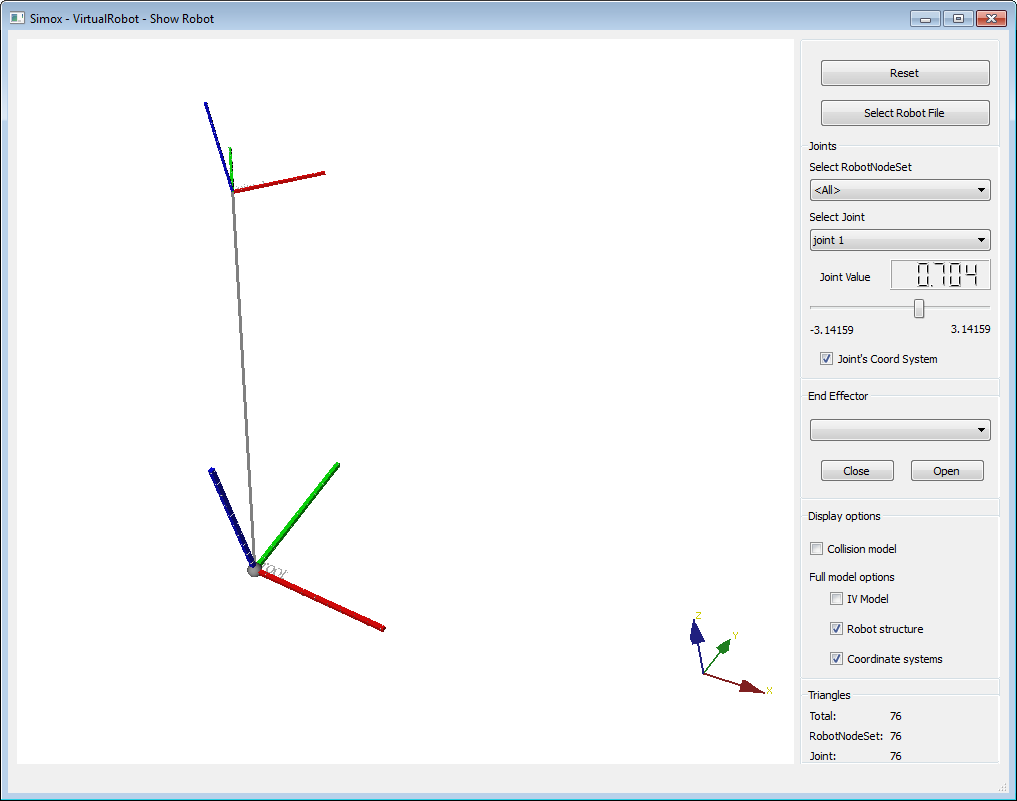
\includegraphics[width=\linewidth]{Tutorial3b}
	\end{minipage}
\end{figure}

\par

\subsubsection{Kinematic Chains}
\par
Now we build a longer kinematic chain by connecting multiple RobotNodes. Some of the nodes are fixed (no Joint tag), while others can be moved indicated by a <Joint type="revolute'> definition. 
\par
\begin{lstlisting}
<Robot Type="DemoRobot" RootNode="root">

   <RobotNode name="root">
     <Child name="joint 1"/>
   </RobotNode>

   <RobotNode name="joint 1">
     <Joint type="revolute">
       <Axis x="0" y="0" z="1"/>
     </Joint>
     <Visualization>
       <File type="Inventor">iv/joint.iv</File>
     </Visualization>
     <Child name="node 1"/>
    </RobotNode>

    <RobotNode name="node 1">
      <Transform>
        <Translation x="0" y="500" z="0"/>
      </Transform>
      <Visualization>
        <File type="Inventor">iv/ball.iv</File>
      </Visualization>
      <Child name="joint 2"/>
    </RobotNode>

    <RobotNode name="joint 2">
      <Joint type="revolute">
        <Axis x="0" y="1" z="0"/>
      </Joint>
      <Visualization>
        <File type="Inventor">iv/joint2.iv</File>
      </Visualization>
      <Child name="node 2"/>
    </RobotNode>

    <RobotNode name="node 2">
      <Transform>
        <Translation x="0" y="0" z="500"/>
      </Transform>
      <Visualization>
        <File type="Inventor">iv/ball.iv</File>
      </Visualization>
      <Child name="joint 3"/>
    </RobotNode>

    <RobotNode name="joint 3">
      <Joint type="revolute">
        <Axis x="1" y="0" z="0"/>
      </Joint>
      <Visualization>
        <File type="Inventor">iv/joint.iv</File>
      </Visualization>
    </RobotNode> 
</Robot>
\end{lstlisting}
\par
\begin{figure}[H]
	\centering
	\begin{minipage} {.45\linewidth}
	  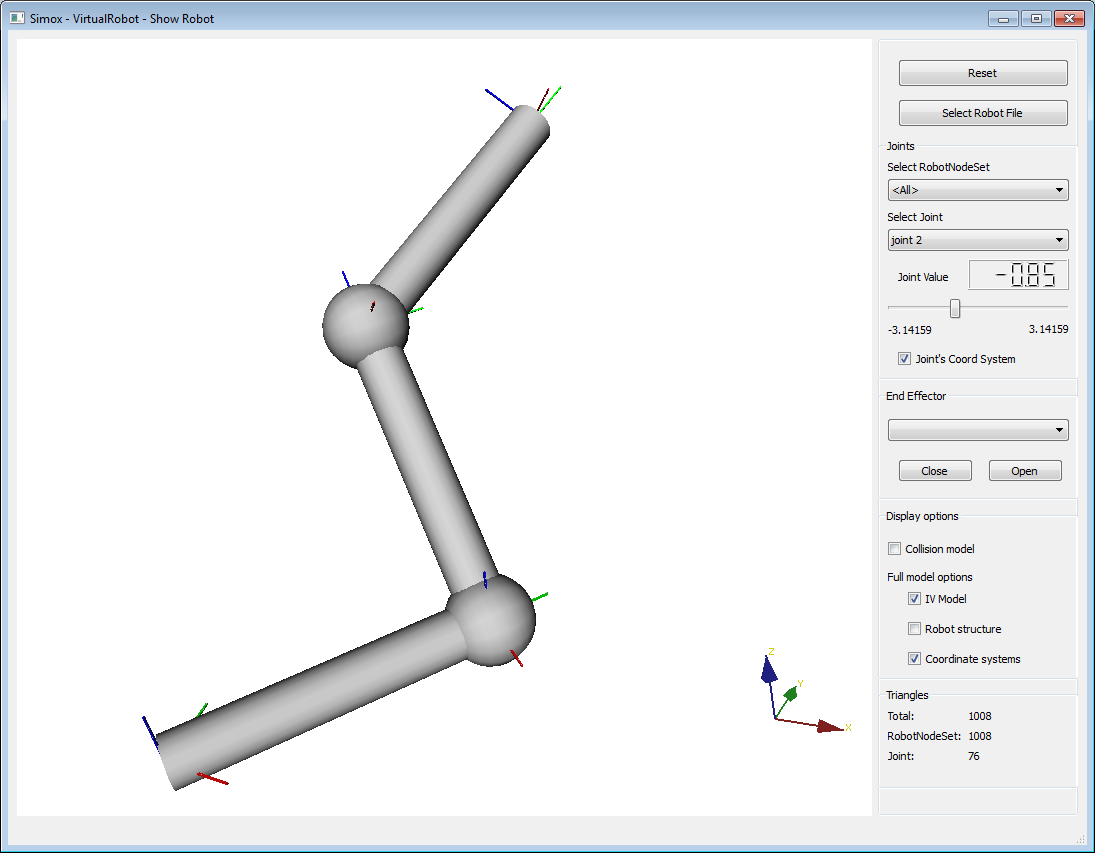
\includegraphics[width=\linewidth]{Tutorial4a}
	\end{minipage}
	%\hspace{.05\linewidth}
	\begin{minipage} {.45\linewidth}
	  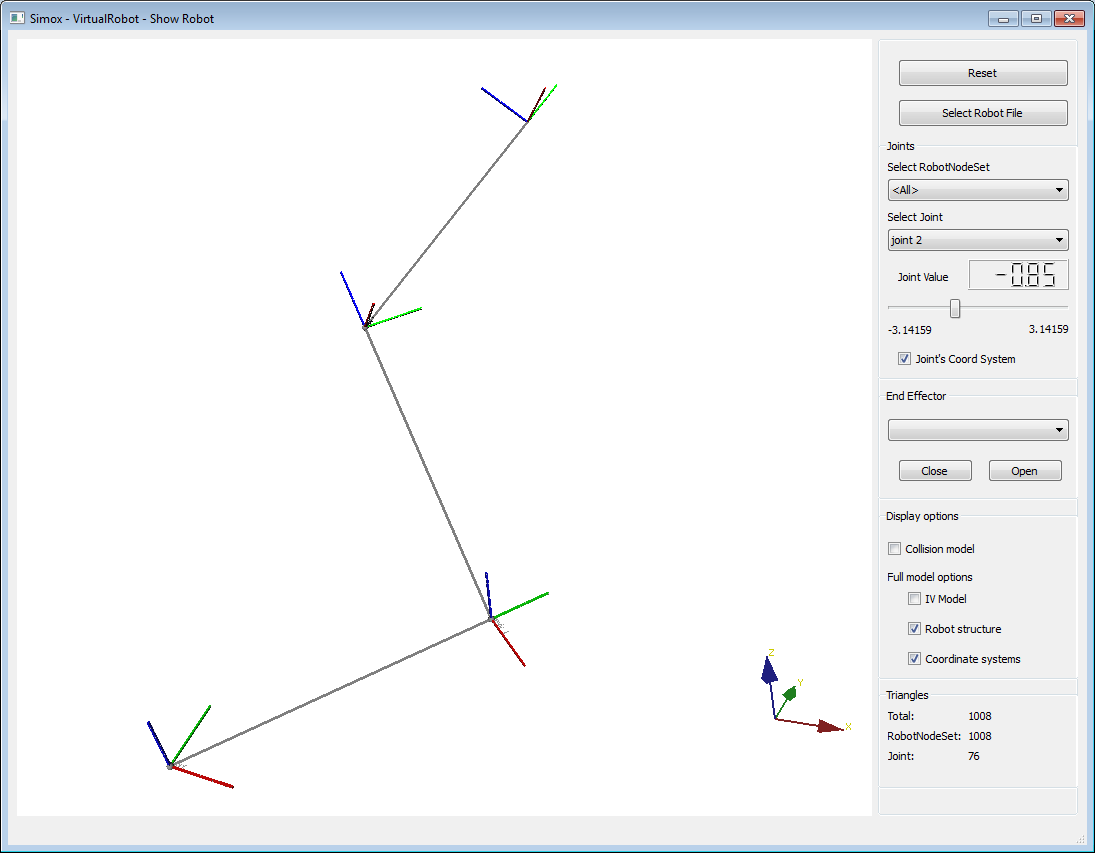
\includegraphics[width=\linewidth]{Tutorial4b}
	\end{minipage}
\end{figure}
\par
\subsubsection{Denavit-Hartenberg Parameters}
\par
A joint can also be definied with Denavit Hartenberg paramters. Therefore the DH tag with the two translational attributes a, d and with both rotational attributes alpha and theta can be used. Please note that you have to specify the units in which the rotation is given (degree or radian). Further, the Limits tag is used to specify the lower and upper joint limits. 
\begin{lstlisting}
<Robot Type="DemoRobot" RootNode="root">

    <RobotNode name="root">
        <Child name="joint 1"/>
    </RobotNode>

    <RobotNode name="joint 1">
        <Joint type="revolute">
        <Limits lo="0" hi="120" units="degree"/>
        </Joint>
        <Visualization>
            <File type="Inventor">iv/joint2.iv</File>
        </Visualization>
        <Child name="node 1"/>
    </RobotNode>

    <RobotNode name="node 1">
        <Transform>
            <DH a="0" d="500" alpha="-90" theta="0" units="degree"/>
        </Transform>
        <Visualization>
            <File type="Inventor">iv/ball.iv</File>
        </Visualization>
        <Child name="joint 2"/>
    </RobotNode>

    <RobotNode name="joint 2">
        <Joint type="revolute">
            <Limits lo="-45" hi="45" units="degree"/>
        </Joint>
        <Visualization>
            <File type="Inventor">iv/joint2.iv</File>
        </Visualization>
        <Child name="node 2"/>
    </RobotNode>

    <RobotNode name="node 2">
        <Transform>
            <DH a="0" d="500" alpha="90" theta="0" units="degree"/>
        </Transform>
    </RobotNode>
</Robot>
\end{lstlisting}
\par
\begin{figure}[H]
	\centering
	\begin{minipage} {.45\linewidth}
	  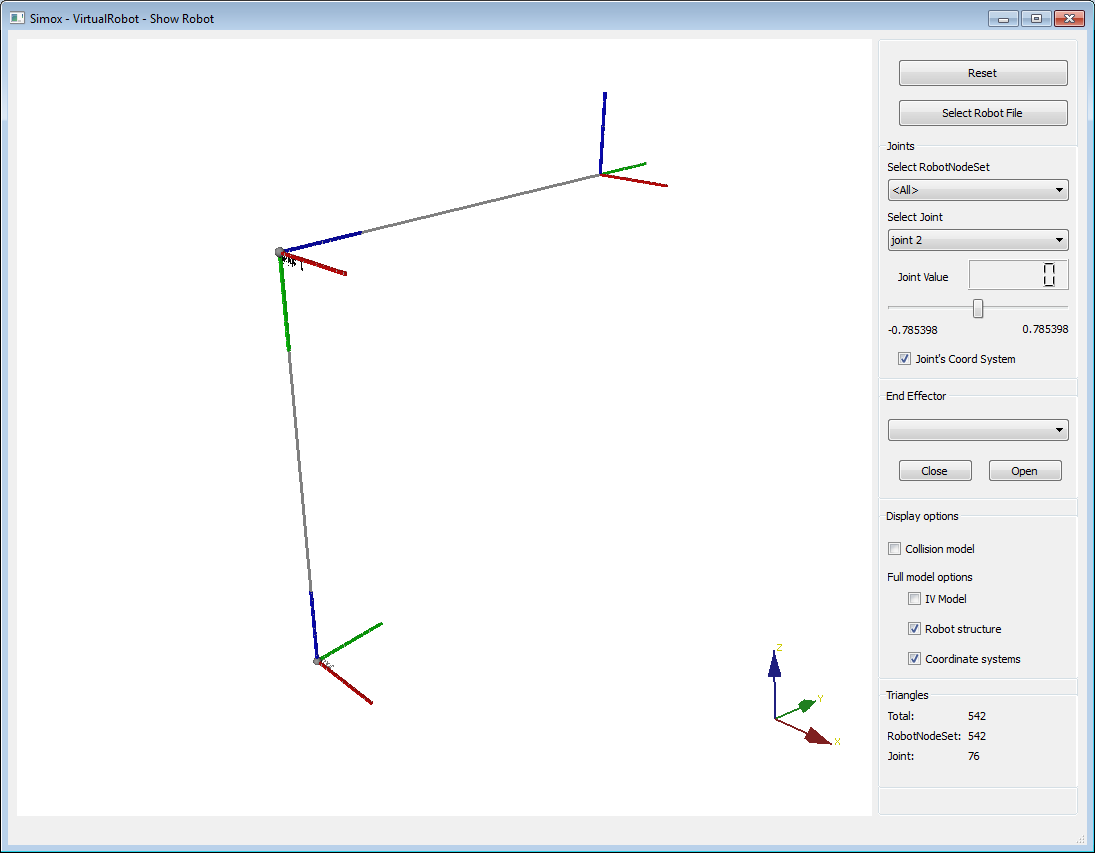
\includegraphics[width=\linewidth]{Tutorial5a}
	\end{minipage}
	%\hspace{.05\linewidth}
	\begin{minipage} {.45\linewidth}
	  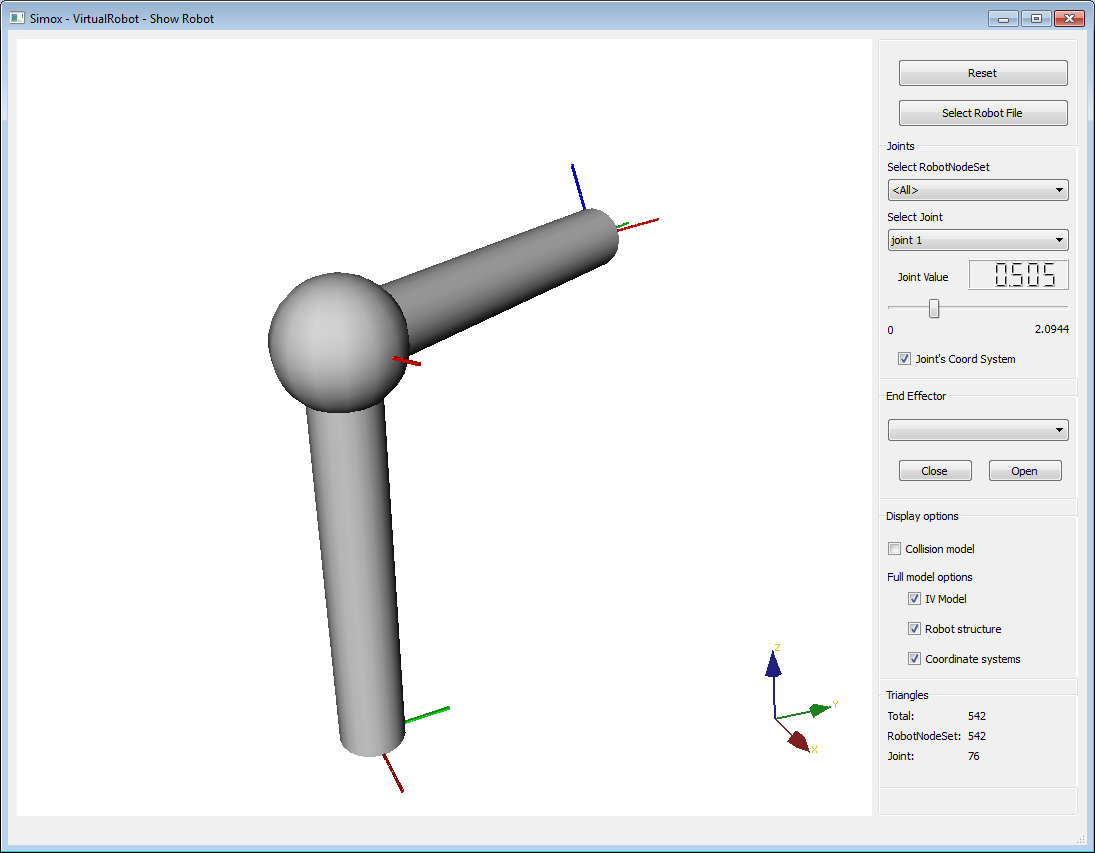
\includegraphics[width=\linewidth]{Tutorial5b}
	\end{minipage}
\end{figure}
\par
\subsubsection{Coordinate Systems}
\par
A RobotNode may cover several transformations.
\par
\begin{description}
  \item[$\bullet$]Transform: This is a fixed transformation which is applied to the initial pose that is passed by the parent of this node.
    \item[$\bullet$] Joint: This transformation depends on the joint type and the current joint value. In classical robot systems this transformation applies a rotation....
\end{description}
   \par
   The GlobalPose of a RobotNode is always the pose that is retrieved after applying all transformations. 
   \par
\subsubsection{Collision Models}
\par
In the following example a finger is modeled with DH parameters. Additionally to the 3D models, the CollisionModel tag is used to specify visualization files that should be used for collision detection. The CollisionModels will automatically be used whenever collision detection is performed, hence usually reduced models are used in order to speed up the collision detection. If the visualization models should be used for collision detection as well you can use the <UseAsCollisionModel/> tag within a <VisualizationModel> definition, in order to avoid loading the 3D model twice. Further, bounding boxes can be automatically created to be used as CollisionModels. Therefore you have to use the attribute boundingbox="true" within the CollisionModel's File tag. 
\par
\begin{lstlisting}
<Robot Type="DemoRobot" RootNode="root">

  <RobotNode name="root">
    <Child name="Finger Joint1"/>
  </RobotNode>

  <RobotNode name="Finger Joint1">
    <Joint type="revolute">
      <Limits unit="degree" lo="-25" hi="25"/>
    </Joint>
    <Visualization enable="true">
      <File type="Inventor">iv/LeftIndexFinger/leftIndexFinger0.iv</File>
    </Visualization>
    <CollisionModel>
      <File type="Inventor">iv/LeftIndexFinger/col_leftIndexFinger0.iv</File>
    </CollisionModel>
    <Child name="BaseToFinger"/>
  </RobotNode>

  <RobotNode name="BaseToFinger">
    <Transform>
      <DH a="14.8" d="0" theta="0" alpha="90" units="degree"/>
    </Transform>
    <Child name="Finger Joint2"/>
  </RobotNode>

  <RobotNode name="Finger Joint2">
    <Transform>
      <DH a="0" d="1.75" theta="0" alpha="0" units="degree"/>
    </Transform>
    <Joint type="revolute">
      <Limits unit="degree" lo="0" hi="90"/>
    </Joint>
    <Visualization enable="true">
      <File type="Inventor">iv/LeftIndexFinger/leftIndexFinger1.iv</File>
    </Visualization>
    <CollisionModel>
      <File type="Inventor">iv/LeftIndexFinger/col_leftIndexFinger1.iv</File>
    </CollisionModel>
    <Child name="Finger Joint3"/>
  </RobotNode>

  <RobotNode name="Finger Joint3">
    <Transform>
      <DH a="25.9" d="0" theta="0" alpha="0" units="degree"/>
    </Transform>
    <Joint type="revolute">
      <Limits unit="degree" lo="0" hi="90"/>
    </Joint>
    <Visualization enable="true">
      <File type="Inventor">iv/LeftIndexFinger/leftIndexFinger2.iv</File>
    </Visualization>
    <CollisionModel>
      <File type="Inventor">iv/LeftIndexFinger/col_leftIndexFinger2.iv</File>
    </CollisionModel>
    <Child name="Finger Joint4"/>
  </RobotNode>

  <RobotNode name="Finger Joint4">
    <Transform>
      <DH a="22" d="0" theta="0" alpha="0" units="degree"/>
    </Transform>
    <Joint type="revolute">
      <Limits unit="degree" lo="0" hi="90"/>
    </Joint>
    <Visualization enable="true">
      <File type="Inventor">iv/LeftIndexFinger/leftIndexFingerTip.iv</File>
    </Visualization>
    <CollisionModel>
      <File type="Inventor">iv/LeftIndexFinger/col_leftIndexFingerTip.iv</File>
    </CollisionModel>
  </RobotNode>

</Robot>
\end{lstlisting}
\par
\begin{figure}[H]
	\centering
	\begin{minipage} {.45\linewidth}
	  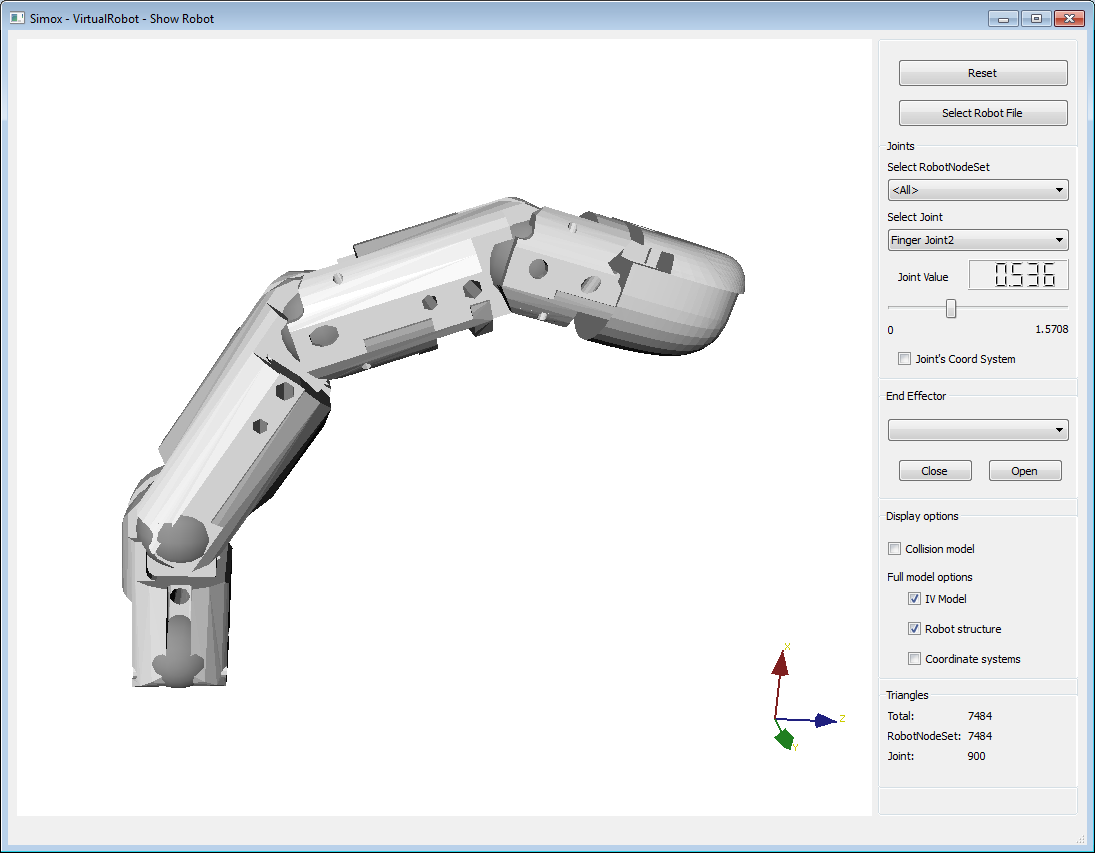
\includegraphics[width=\linewidth]{Tutorial6a}
	\end{minipage}
	%\hspace{.05\linewidth}
	\begin{minipage} {.45\linewidth}
	  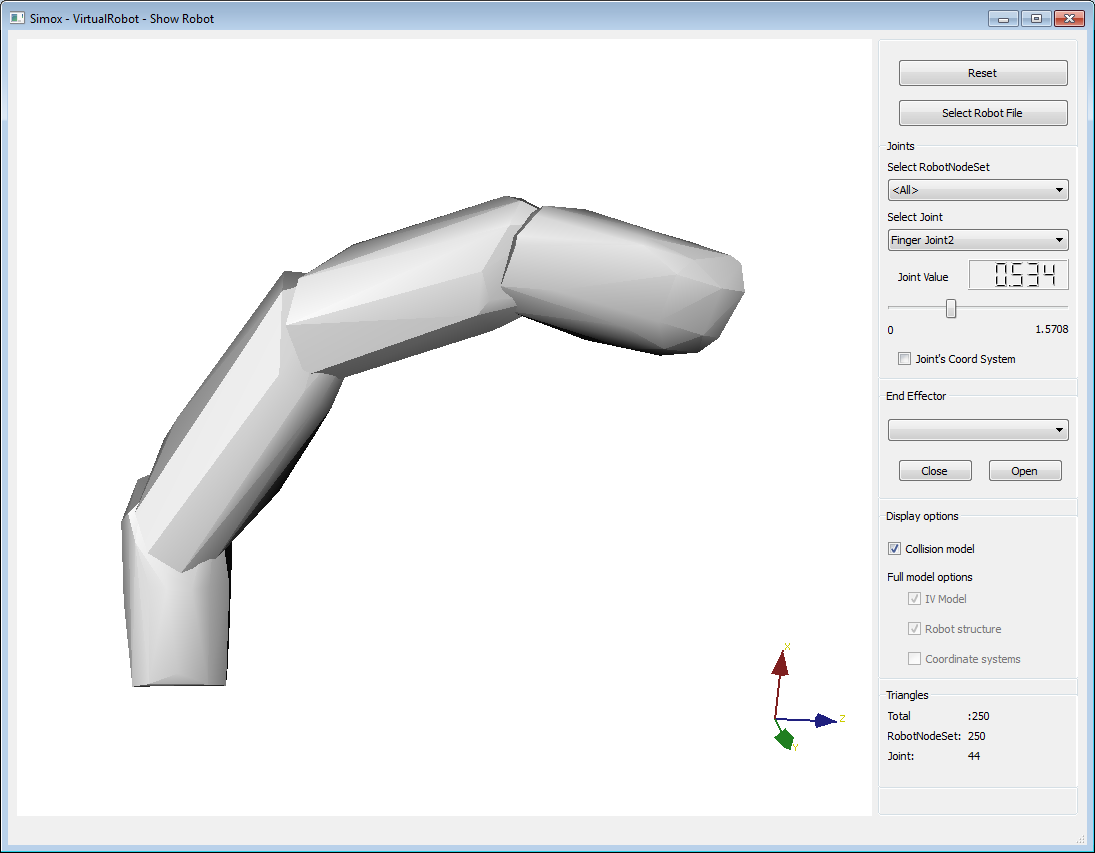
\includegraphics[width=\linewidth]{Tutorial6b}
	\end{minipage}
\end{figure}
\par
\subsubsection{Multiple Files}
\par
When building complex robot models, usually several parts of the robot can be separated. In order to reflect this fact, robots can be assembled from multiple files. In the following example a robot imports another robot and connects the root node to Joint1. Further, you can see how coordinate axis visualizations are enabled and that a RobotNode can have multiple children, allowing to build tree-like kinematic structures. 
\par
\begin{lstlisting}
<Robot Type="robot1" RootNode="Joint1">

    <RobotNode name="Joint1">
        <Joint type="revolute">
            <Limits unit="degree" lo="-90" hi="45"/>
        </Joint>
        <!-- Imports the kinematic structure form otherRobot.xml and adds otherRobot's rootnode as a child to this node -->
        <ChildFromRobot>
            <File importEEF="true">robot_howto7b.xml</File>
        </ChildFromRobot>
        <Child name="node2.1"/>
    </RobotNode>

    <RobotNode name="node2.1">
        <Transform>
            <DH a="0" d="500" theta="-30" alpha="0" units="degree"/>
        </Transform>
    </RobotNode>

</Robot>
\end{lstlisting}
\par
The second file (robot howto7b.xml) looks like this. The file can also be used as a independent robot model. 
 \par
 \begin{lstlisting}
 <Robot Type="robot2" RootNode="node1">
 
  <RobotNode name="node1">
    <Child name="node2"/>
    <Child name="node3"/>
  </RobotNode>
 
  <RobotNode name="node2">
    <Transform>
        <Translation x="0" y="500" z="0"/>
    </Transform>
    <Visualization enable="true">
      <CoordinateAxis type="Inventor" enable="true" scaling="1" text="TCP1"/>
    </Visualization>
  </RobotNode>
 
  <RobotNode name="node3">
    <Transform>
        <Translation x="0" y="-500" z="0"/>
    </Transform>
    <Visualization enable="true">
      <CoordinateAxis type="Inventor" enable="true" scaling="1" text="TCP2"/>
    </Visualization>
  </RobotNode>
 
 </Robot>
 \end{lstlisting}
 \par
 \begin{figure}[H]
 	\centering
 	\begin{minipage} {.45\linewidth}
 	  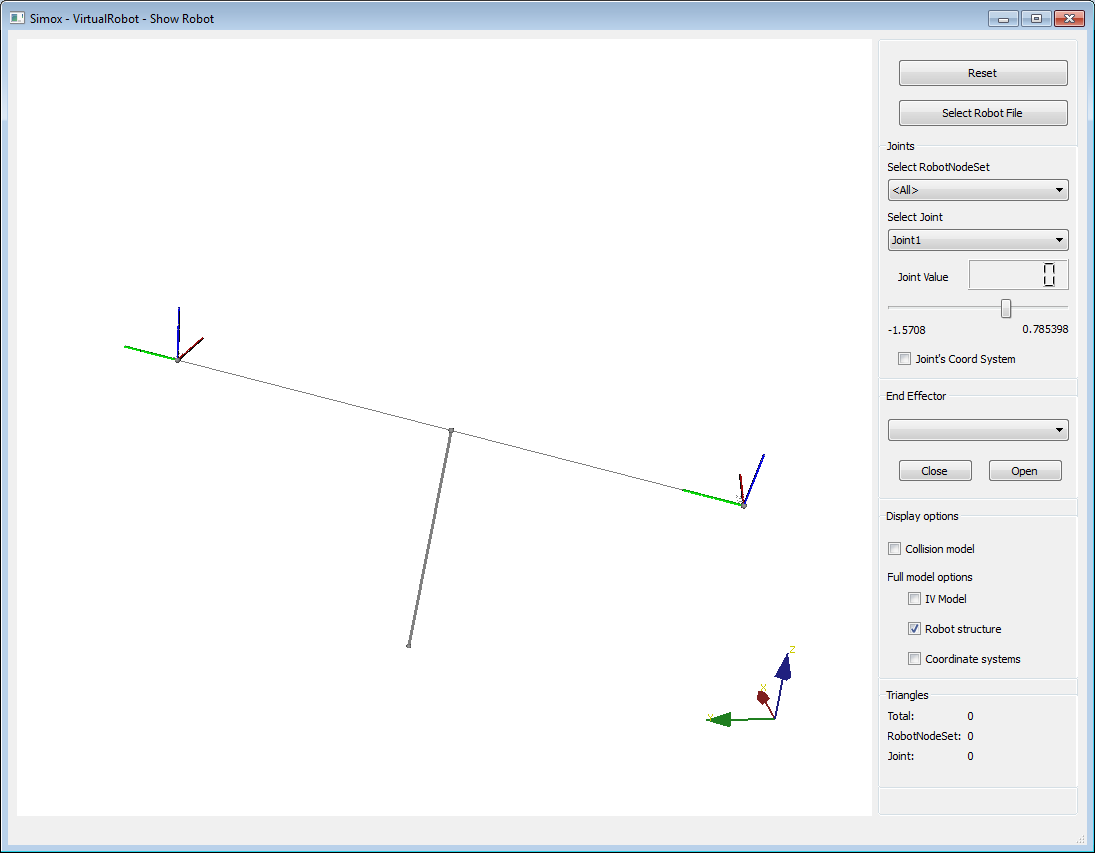
\includegraphics[width=\linewidth]{Tutorial7}
 	\end{minipage}
 	%\hspace{.05\linewidth}
 	\begin{minipage} {.45\linewidth}
 	  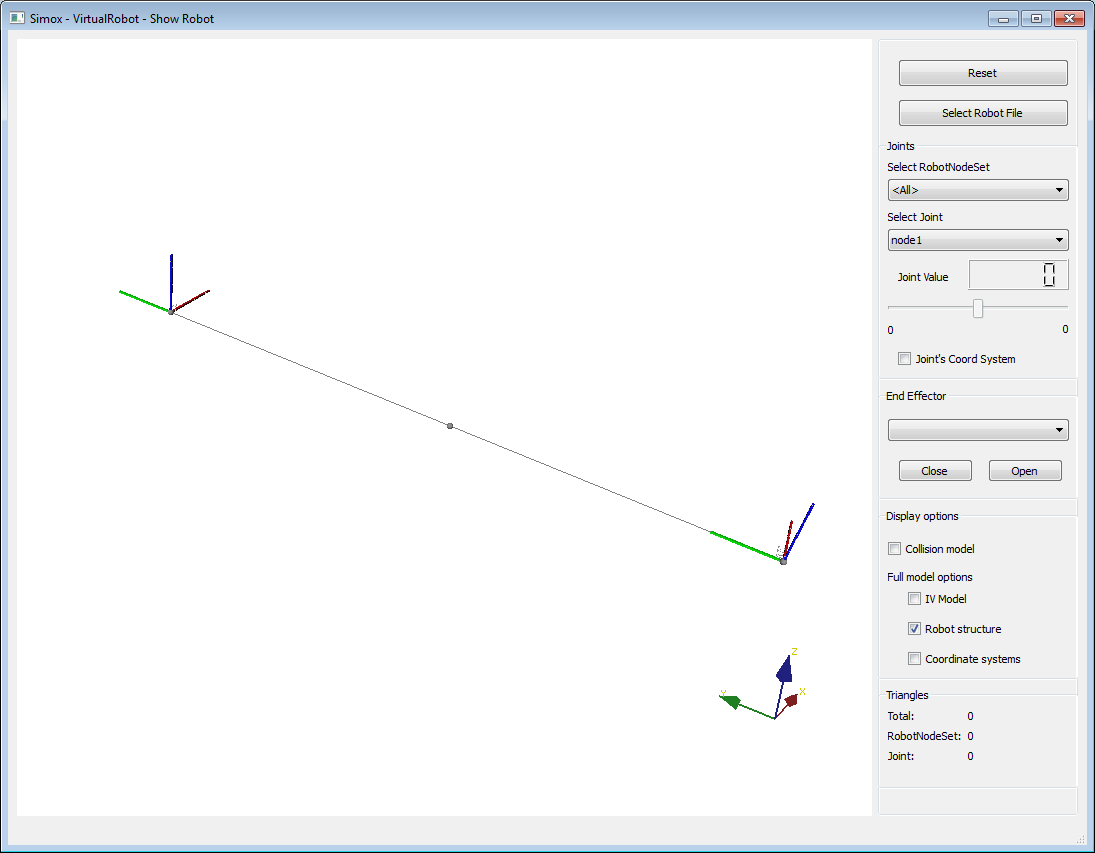
\includegraphics[width=\linewidth]{Tutorial7b}
 	\end{minipage}
 \end{figure}
 \par
\subsubsection{Robot Node Sets}
\par
In VirtualRobot so-called RobotNodeSets are used to group joints or to define kinematic chains. A robot node set consists of a set of robot nodes and optionally
\begin{description}
\item[$\bullet$] A root node, defining the topmost node which has to be updated in order to internally re-compute the kinematic structure, e.g. when changing joint values. If not given, the root of the robot is used.
\item[$\bullet$]A RobotNode defining the Tool Center Point (TCP) coordinate system. This node specifies a TCP for a kinematic chain. The following example shows how a RobotNodeSet is defined. Please note that the order of the joint definitions is preserved for later use. 
\end{description}
\par
\begin{lstlisting}
<Robot Type="DemoRobot" RootNode="root">

   <RobotNode name="root">
     <Child name="joint 1"/>
   </RobotNode>

   <RobotNode name="joint 1">
     <Joint type="revolute">
        <Axis x="0" y="0" z="1"/>
     </Joint>
     <Visualization>
       <File type="Inventor">iv/joint.iv</File>
     </Visualization>
     <Child name="node 1"/>
   </RobotNode>

  <RobotNode name="node 1">
     <Transform>
         <Translation x="0" y="500" z="0"/>
     </Transform>
     <Visualization>
       <File type="Inventor">iv/ball.iv</File>
     </Visualization>
     <Child name="joint 2"/>
   </RobotNode>

   <RobotNode name="joint 2">
     <Joint type="revolute">
       <Axis x="0" y="1" z="0"/>
     </Joint>
     <Visualization>
       <File type="Inventor">iv/joint2.iv</File>
     </Visualization>
     <Child name="node 2"/>
   </RobotNode>

   <RobotNode name="node 2">
       <Transform>
           <Translation x="0" y="0" z="500"/>
       </Transform>
       <Visualization>
           <File type="Inventor">iv/ball.iv</File>
       </Visualization>
       <Child name="joint 3"/>
   </RobotNode>

   <RobotNode name="joint 3">
       <Joint type="revolute">
         <Axis x="1" y="0" z="0"/>
       </Joint>
       <Visualization>
         <File type="Inventor">iv/joint.iv</File>
       </Visualization>
       <Child name="tcp"/>
   </RobotNode>

   <RobotNode name="tcp">
       <Transform>
         <Translation x="0" y="500" z="0"/>
       </Transform>
       <Visualization>
         <File type="Inventor">iv/ball.iv</File>
       </Visualization>
   </RobotNode>

   <RobotNodeSet name="my kinematic chain" kinematicRoot="joint1" tcp="tcp">
     <Node name="joint 1"/>
     <Node name="joint 2"/>
     <Node name="joint 3"/>
   </RobotNodeSet>

</Robot>
\end{lstlisting}
\par
\begin{figure}[H]
	\centering
	\begin{minipage} {.45\linewidth}
	  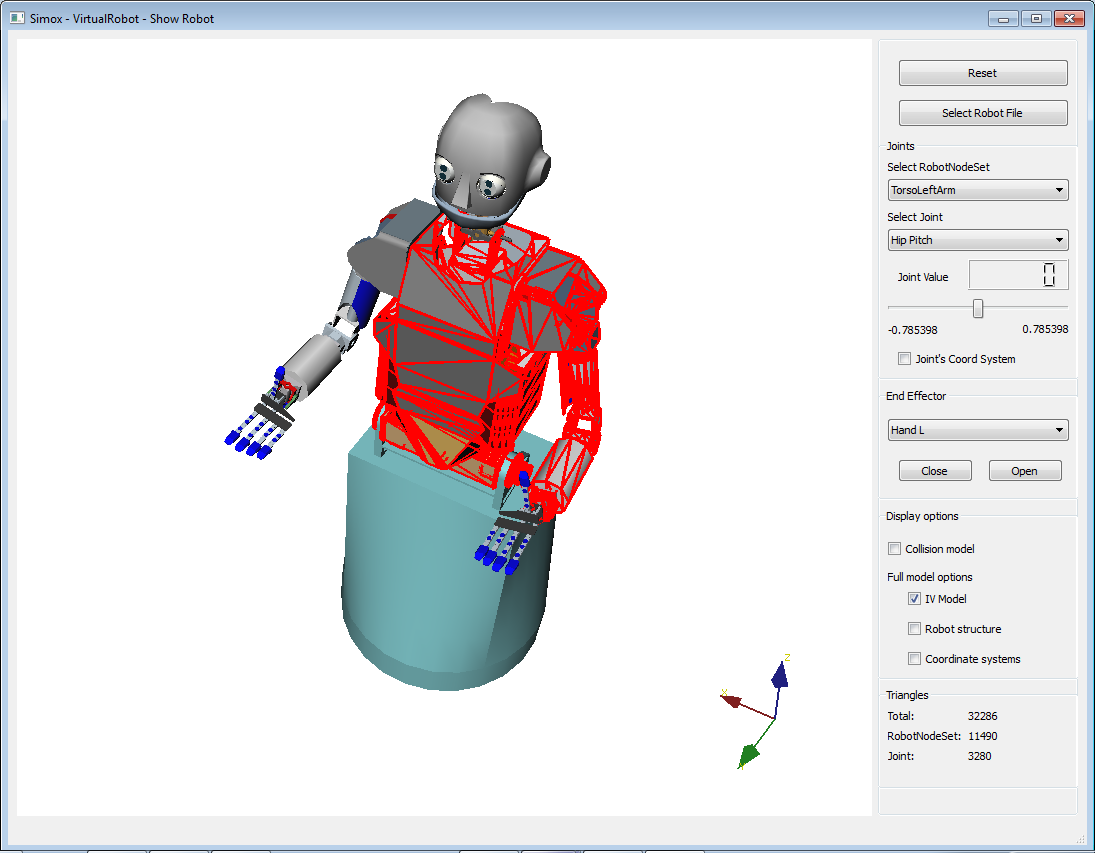
\includegraphics[width=\linewidth]{Tutorial8}
	\end{minipage}
	%\hspace{.05\linewidth}
	\begin{minipage} {.45\linewidth}
	  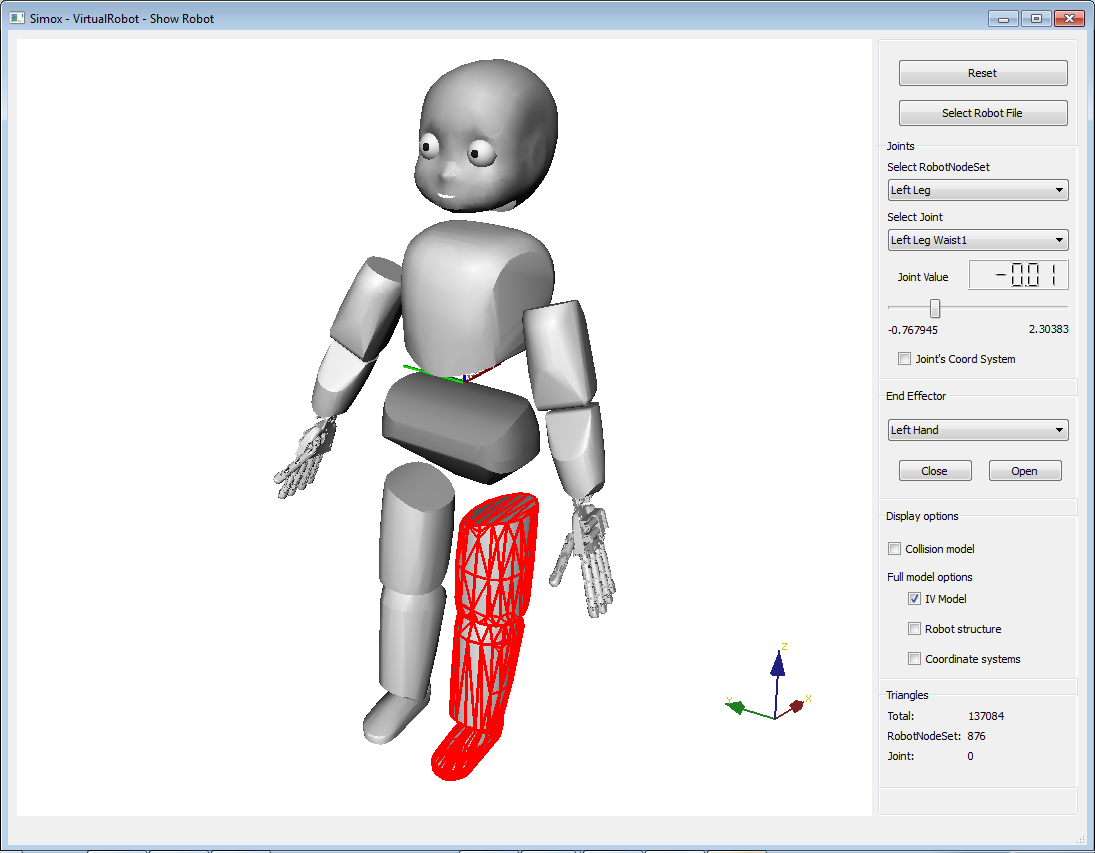
\includegraphics[width=\linewidth]{Tutorial8b}
	\end{minipage}
\end{figure}
\par
\subsubsection{End Effector Definitions}
When complex robot systems, such as humanoid robots, should be modeled a logical definition of their end-effectors is helpful especially in the context of grasp and manipulation planning. In order to access the robot's end-effector conveniently it can be defined in the robot's XML definition. An end-effector is a logical collection of static RobtoNodes and so-called actors which are lists of RobotNodes defining a finger. Please note that the RobotNodes have to be defined within the robot's XML definition. The static parts are not moved when the end-effector is accessed (e.g. closed or opened), whereas the actors are moved. As shown in the example below, actors consist of a set of RobotNodes and for each node several options can be specified:
\begin{itemize}
  \item name: The name string of the RobotNode. This node must be present in the robot's definition. 
  \item considerCollisions: Here the behavior for collision detection can be adjusted. Possible options are 
  \begin{itemize}
    \item all (standard): Collisions between the static part and the RobotNode and between other actors and the RobotNode are considered. 
    \item none The node is not considered for collision detection. E.g. when closing the hand an actor will not stop if this node is in collision. 
    \item actors: Collisions between the static part of teh hand and the node are not considered, but collisions between other actors and the RobotNode are. 
    \item static: Only collisions between this node and the static part of the end-effector are considered, while collision between this node and other actors are not considered. 
  \end{itemize}

  \item direction: Here the moving direction can be inverted by setting this value to -1. Further, the relative speed of moving can be adjusted (the standard value is 1). 

\end{itemize}
\begin{lstlisting}
<Robot Type="iCub Left Hand" RootNode="root">
    ...
    <Endeffector name="Left Hand" base="Left Hand Init" tcp="Left Arm TCP" gcp="Left Arm GCP">
        <Preshape name="Grasp Preshape">
            <Node name="Left Hand Thumb Joint1" unit="radian" value="1.3"/>
        </Preshape>

        <Static>
            <Node name="Left Hand Palm"/>
            <Node name="Left Hand Thumb Joint1"/>
        </Static>

        <Actor name="Left Hand Thumb">
            <Node name="Left Hand Thumb Joint2" considerCollisions="Actors"/>
            <Node name="Left Hand Thumb Joint3" considerCollisions="All"/>
            <Node name="Left Hand Thumb Joint4" considerCollisions="All"/>
        </Actor>
        <Actor name="Left Hand Index">
            <Node name="Left Hand Index Joint2" considerCollisions="Actors"/>
            <Node name="Left Hand Index Joint3" considerCollisions="All"/>
            <Node name="Left Hand Index Joint4" considerCollisions="All"/>
        </Actor>
        <Actor name="Left Hand Middle">
            <Node name="Left Hand Middle Joint2" considerCollisions="Actors"/>
            <Node name="Left Hand Middle Joint3" considerCollisions="All"/>
            <Node name="Left Hand Middle Joint4" considerCollisions="All"/>
        </Actor>
        <Actor name="Left Hand Ring">
            <Node name="Left Hand Ring Joint2" considerCollisions="Actors"/>
            <Node name="Left Hand Ring Joint3" considerCollisions="All"/>
            <Node name="Left Hand Ring Joint4" considerCollisions="All"/>
        </Actor>
        <Actor name="Left Hand Pinky">
            <Node name="Left Hand Pinky Joint2" considerCollisions="Actors"/>
            <Node name="Left Hand Pinky Joint3" considerCollisions="All"/>
            <Node name="Left Hand Pinky Joint4" considerCollisions="All"/>
        </Actor>
    </Endeffector>
</Robot>
\end{lstlisting}
\par
\begin{figure}[H]
	\centering
	\begin{minipage} {.45\linewidth}
	  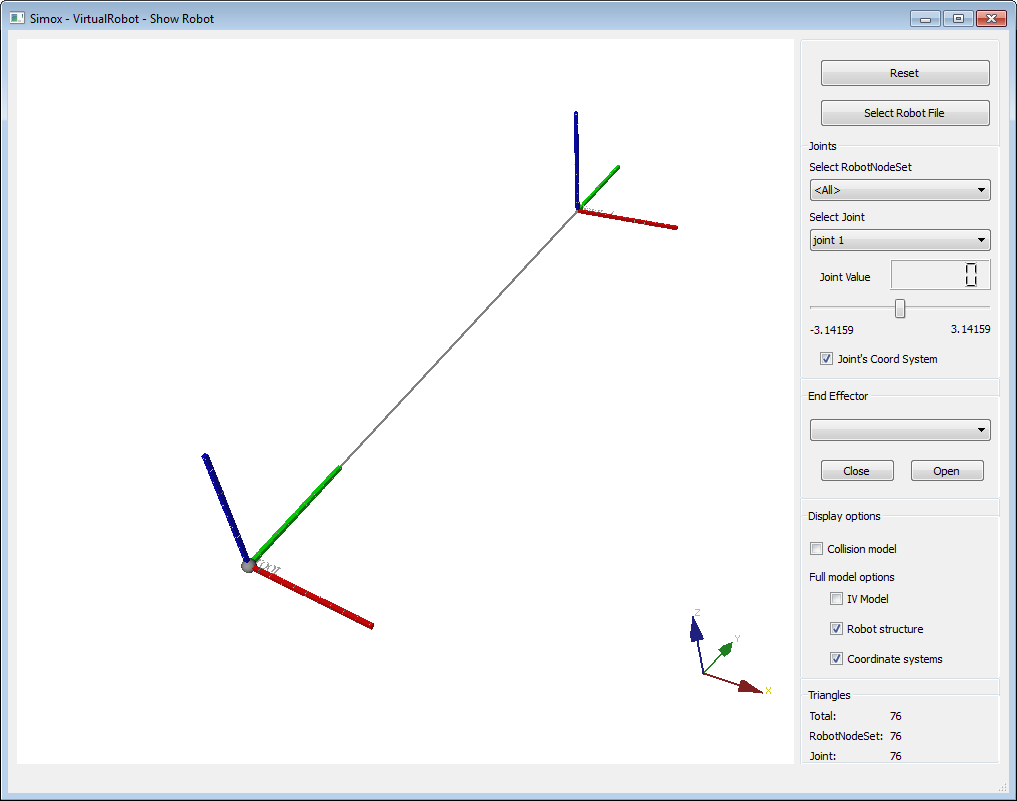
\includegraphics[width=\linewidth]{Tutorial3a}
	\end{minipage}
	%\hspace{.05\linewidth}
	\begin{minipage} {.45\linewidth}
	  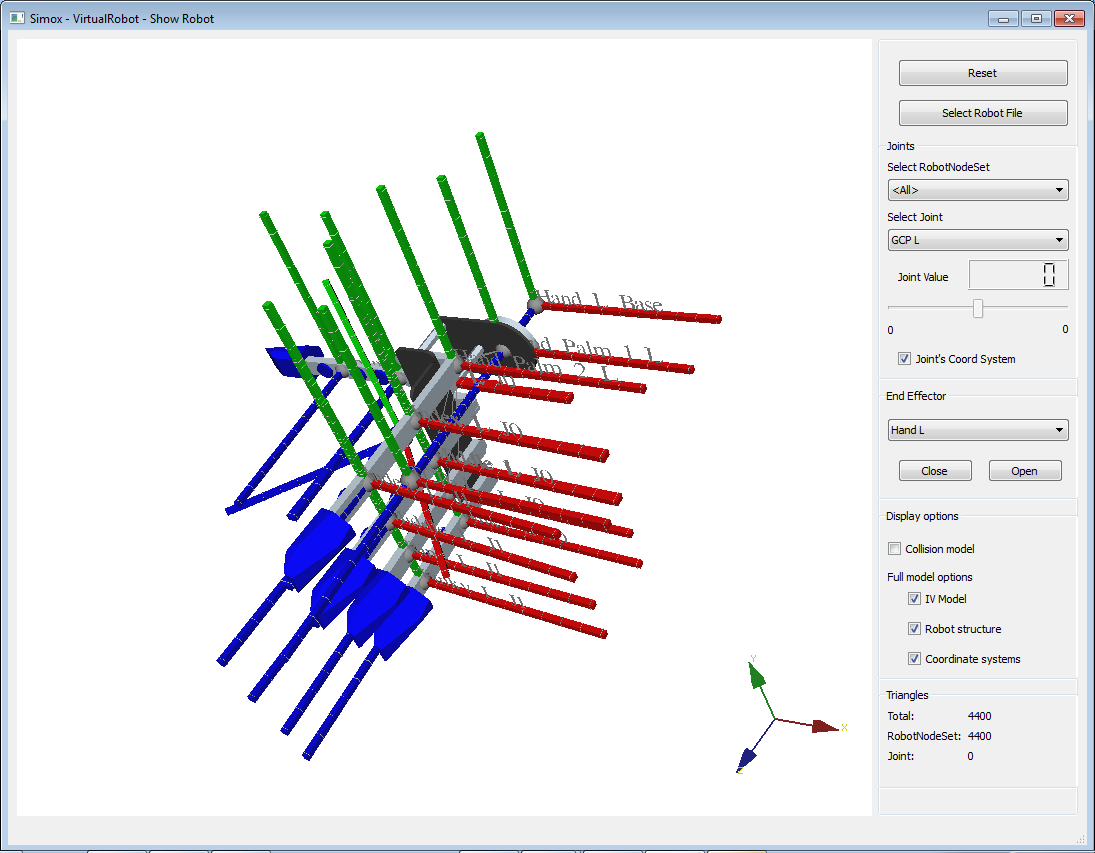
\includegraphics[width=\linewidth]{Tutorial9b}
	\end{minipage}
\end{figure}
\begin{figure}[H]
	\centering
	\begin{minipage} {.45\linewidth}
	  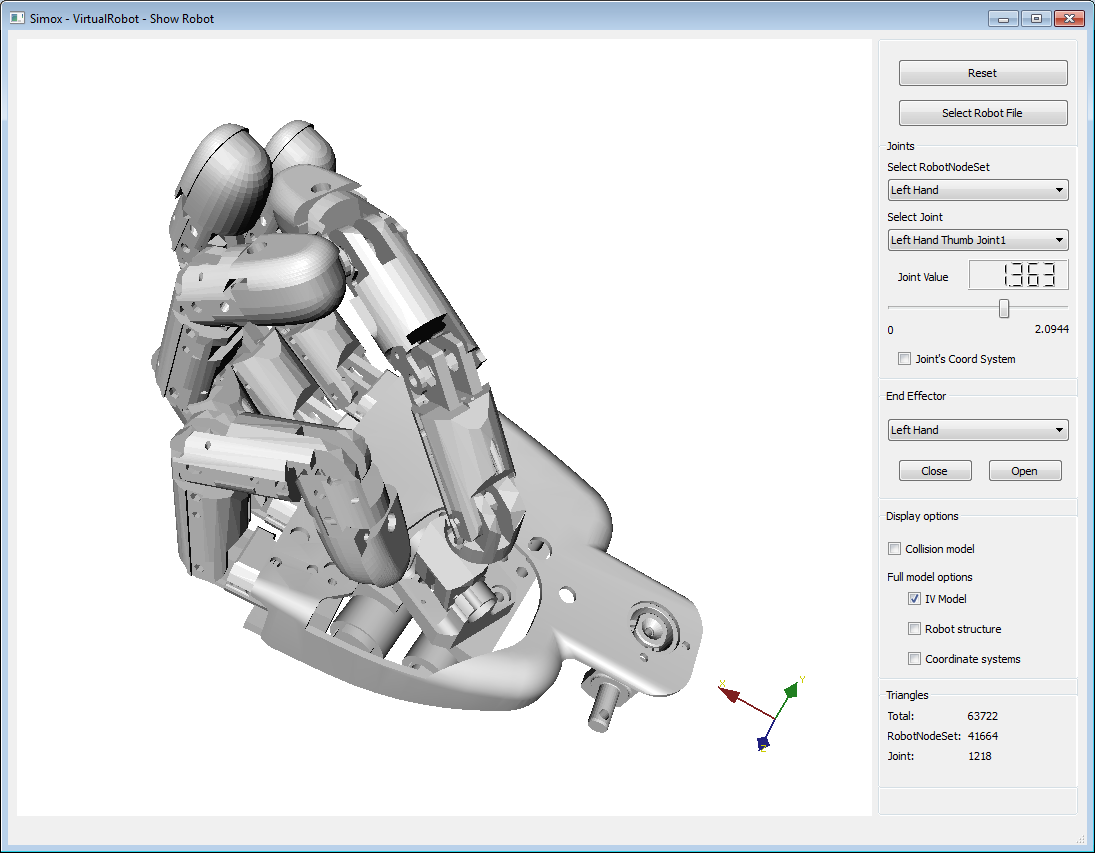
\includegraphics[width=\linewidth]{Tutorial9c}
	\end{minipage}
	%\hspace{.05\linewidth}
\end{figure}
\par
\subsubsection{Objects and Scenes}
\par
Scenes can be defined via XML files, allowing to specify a setup for robots and obstacles. Further, configurations can be defined allowing to easily access them later on. The following tags can be used: 
\begin{itemize}
  \item Robot: Define a robot with a name and an optional initial configuration initConfig. 

  \begin{itemize}
    \item The File tag specifies the robot's XML file from which the model should be loaded. 
    \begin{itemize}
    \item Files are searched in all dataPaths which are specified in VirtualRobot::RuntimeEnvironment (initially some simox-related standard data paths are set). 
    \item Optional the attribute path can set to absolute or relative, in order to force absolute or relative (w.r.t. the scene file) path names. 
    \end{itemize}
    \item Multiple Configurations can be defined, which can be accessed via their name strings. 
    \begin{itemize}
    \item A Configuration is a list of RobotNodes with corresponding joint values. 
    \end{itemize}
    \item A GlobalPose tag encapsulates a Transfrom tag which can be used to position the robot in the scene. 
  \end{itemize}

  \item Obstacles can be loaded from files. Here the same syntax is provided as when setting Visualization tags for a RobotNode: 
  \begin{itemize}
       \item The type of 3d model must be specified in the File tag. Again the file names are searched in the paths, defined in VirtualRobot::RuntimeEnvironment. Optionally the attributes path='absolute' or path='relative' allow to specify absolute or scene-file-relative file names.
      \item A GlobalPose can be used to position the object.
      \item The <UseAsCollisionModel/> tag ensures that the visualization model is used as a collision model.
  \end{itemize}
\item A ManipulationObject is basically a 3d object with predefined grasping information. These objects can also be positioned via the GlobalPose tag. 
\end{itemize}
\par
\begin{lstlisting}
<Scene name="Armar3Scene">

    <Robot name="Armar3" initConfig="start">
        <File>robots/ArmarIII/ArmarIII.xml</File>
        <Configuration name="start">
            <Node name="Shoulder 1 L" unit="radian" value="-0.85"/>
            <Node name="Shoulder 2 L" unit="radian" value="-0.8"/>
            <Node name="Upperarm L" unit="radian" value="-0.85"/>
            <Node name="Shoulder 1 R" unit="radian" value="-0.85"/>
            <Node name="Shoulder 2 R" unit="radian" value="0.8"/>
            <Node name="Upperarm R" unit="radian" value="0.85"/>
        </Configuration>
        <GlobalPose>
            <Transform>
                <Translation x="1000" y="0" z="0"/>
            </Transform>
        </GlobalPose>
    </Robot>

    <Robot name="Armar3b">
        <File>robots/ArmarIII/ArmarIII.xml</File>           
    </Robot>

    <Obstacle name="Box">
        <Visualization>
            <File type="Inventor">objects/iv/box1000x500x300.iv</File>
            <UseAsCollisionModel/>
        </Visualization>
        <GlobalPose>
            <Transform>
                <Translation x="9000" y="1500" z="150"/>
                <rollpitchyaw units="degree" roll="0" pitch="0" yaw="90"/>
            </Transform>
        </GlobalPose>
    </Obstacle>

    <ManipulationObject name="Plate">
        <File>objects/plate.xml</File>    
        <GlobalPose>
            <Transform>
                <Translation x="-250" y="0" z="600"/>
                <rollpitchyaw units="degree" roll="90" pitch="0" yaw="90"/>
            </Transform>
        </GlobalPose>
    </ManipulationObject>

</Scene>
\end{lstlisting}
\par
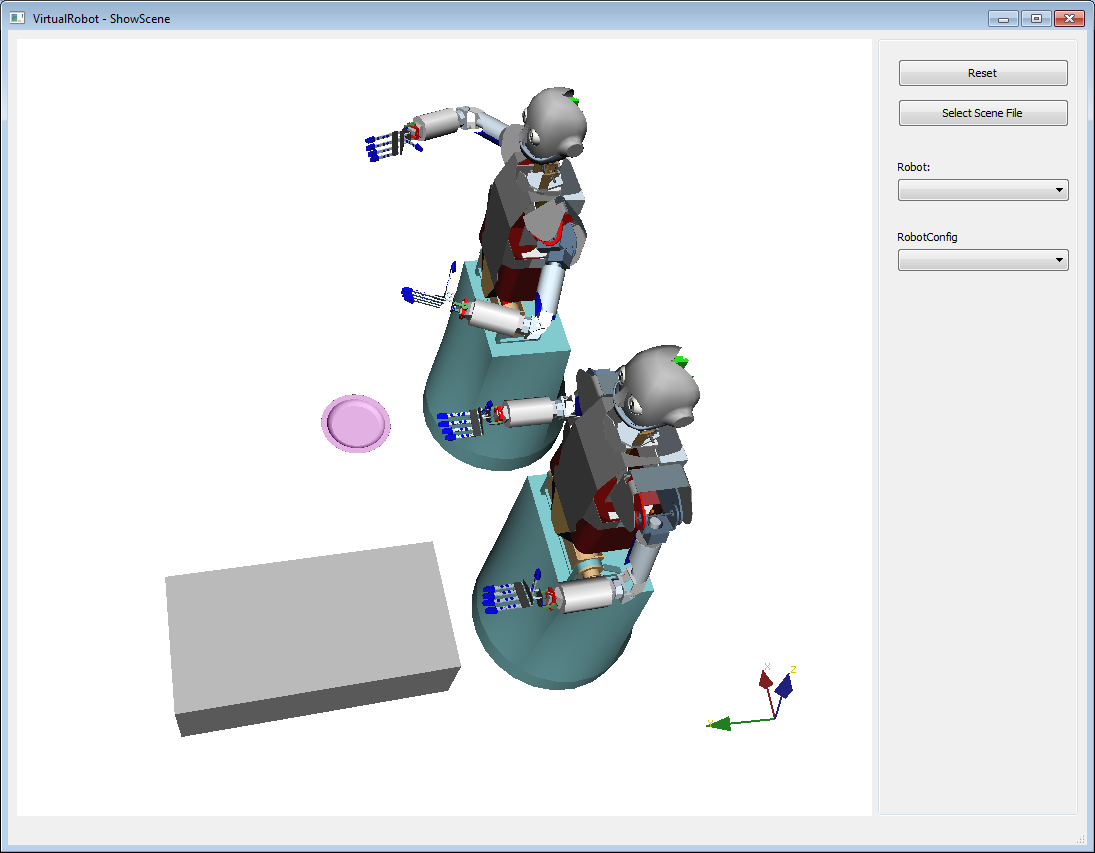
\includegraphics[width=\textwidth]{Tutorial10}
\par
\subsection{Virtual Robot: The robot library}
Once a robot and/or scene information are created , one can load and access the data via the VirtualRobot library. The C++ API offers convenient access, which is described in the following sections. 
\par
\subsubsection{Preliminaries}
We start with a brief introduction, showing how some internals are organized 
\par
\subsubsection*{Shared Pointers}
Simox uses boost's shared pointers (also called smart pointers) in order to avoid memory leaks. If you are not familiar with shared pointer have a look at the official boost reference page: http://boost.org/libs/smart\_ptr/smart\_ptr.htm. In order to achieve a better readability of the source code, the following commonly used typedef is used for defining pointers: 
\begin{lstlisting}
typedef boost::shared_ptr<class> classPtr;
\end{lstlisting}
Hence the pointer to an instance of a VirtualRobot::Robot object can be written as VirtualRobot::RobotPtr (instead of the long version boost::shared\_ptr<VirtualRobot::Robot>). Please note, that you never need to delete a pointer, since the smart pointer's reference counting system does this for you. 
\subsubsection*{Matrices and Poses}
Internally poses (which consist of a location and orientation) are handled with homogeneous 4x4 matrices. Therefore, the Eigen::Matrix4f type is used. Further information can be found at http://eigen.tuxfamily.org. 
\par
\subsubsection*{Namespaces}
In Simox three namespaces are defined: 
\begin{itemize}
\item VirtualRobot
\item Saba
\item GraspStudio
\end{itemize}
\subsubsection*{VirtualRobot::RuntimeEnvironmentt}
Several paths to data files are defined during the compilation process (E.g. the main data directory SimoxDir/VirtualRobot/data containing robot models, obstacles and precomputed grasp sets). Further, it is possible to add custom paths to the list of data paths in order to avoid absolute path names during execution. A data path can be set with 
\begin{lstlisting}
VirtualRobot::RuntimeEnvironment::addDataPath("/path/to/add");
\end{lstlisting}
And the list of all paths can be retrieved with 
\begin{lstlisting}
std::vector<std::string> allDataPaths = VirtualRobot::RuntimeEnvironment::getDataPaths();
\end{lstlisting}
In order to specify search paths from the command line, the build in command line parsing of Simox can be used. When starting your application with 
\begin{lstlisting}
./yourBinary --data-path "my/path/to/data"
\end{lstlisting}
the specified path will automatically added to the list of search paths when you process the command line as follows: 
\begin{lstlisting}
int main(int argc, char *argv[])
{
    VirtualRobot::RuntimeEnvironment::processCommandLine(argc,argv);
    // ...
}
\end{lstlisting}
When you want to pass custom flags to your program you can use the RuntimeEnvironment methods as well. Have a look at the following example: 
\begin{lstlisting}
int main(int argc, char *argv[])
{
    VirtualRobot::RuntimeEnvironment::considerKey("robot");
    VirtualRobot::RuntimeEnvironment::processCommandLine(argc,argv);
    VirtualRobot::RuntimeEnvironment::print();
    std::string filename(VR_BASE_DIR "/data/robots/ArmarIII/ArmarIII.xml");
    if (VirtualRobot::RuntimeEnvironment::hasValue("robot"))
    {
        std::string robFile = VirtualRobot::RuntimeEnvironment::getValue("robot");
        // check if the path is absolute or if can be created 
        if (VirtualRobot::RuntimeEnvironment::getDataFileAbsolute(robFile))
            filename = robFile;
    }
    cout << "Using robot file " << filename << endl;
    //...
}
\end{lstlisting}
\subsubsection*{VirtualRobot::SceneObject}
All objects in VirtualRobot that may have a visualization (e.g. Robots, RobotNodes, Obstacles) are derived from the class SceneObject, which allows a hierarchical scene representation. SceneObjects may have children which are automatically updated/positioned when the parent is moved.
\subsubsection{Accessing a Robot}
A robot can be loaded as follows:
\begin{lstlisting}
VirtualRobot::RobotPtr robot;
try
{
    robot = VirtualRobot::RobotIO::loadRobot(filename);
} catch (VirtualRobot::VirtualRobotException &e)
{
    std::cout << "Error: " << e.what() << std::endl;
}
\end{lstlisting}
\subsubsection*{RobotNodes: Accessing joints}
A RobotNode can be retrieved with
\begin{lstlisting}
VirtualRobot::RobotNodePtr rn = robot->getRobotNode("name of robot node");
\end{lstlisting}
The joint value can be set with 
\begin{lstlisting}
rn->setJointValue(myJointValueRadian);
\end{lstlisting}
The joint value can be retrieved with
\begin{lstlisting}
float v =  rn->getJointValue();
\end{lstlisting}
The pose of the RobotNode's coordiante system can be retrieved with
\begin{lstlisting}
Eigen::Matrix4f p = rn->getGlobalPose();
\end{lstlisting}
\subsubsection*{RobotConfig: Configurations of the robot}
A RobotConfig represents a name,value map of joint values.
\begin{lstlisting}
// Consider all RobotNodes
RobotConfigPtr c = robot->getConfig();
c->setConfig("joint 1", 0.5f);
robot->setConfig(c);
\end{lstlisting}
\subsubsection*{RobotNodeSets}
A set of RobotNodes defined in the robot's XML file can be accessed with
\begin{lstlisting}
VirtualRobot::RobotNodeSetPtr rns = robot->getRobotNodeSet("name of robot node set");
std::vector<float> jointValues = rns->getJointValues();
rns->setJointValues(jointValues);
\end{lstlisting}
When a kinematic chain is defined via a RobotNodeSet, its TCP node can be retrieved: 
\begin{lstlisting}
VirtualRobot::RobotNodePtr tcp = rns->getTCP();
\end{lstlisting}
\subsubsection*{Coordinate Transformations}
Usually poses of objects and RobotNodes are given in the global coordinate system, but they can be transformed to local coordinate systems of other objects and vice versa. E.g. an object's position can be transformed to the hand coordinate system. 
\begin{lstlisting}
Eigen::Matrix4f localObjectPose robotNodeHand->toLocalCoordinateSystem(poseObjectGlobal);
\end{lstlisting}
In the following example the visually localized pose of a hand, given in the camera coordinate system, located in the left eye, is transformed to the global coordinate system: 
\begin{lstlisting}
Eigen::Matrix4f globalHandPose robotNodeEyeLeft->toGlobalCoordinateSystem(localHandPose);
\end{lstlisting}
\subsubsection*{End Effectors}
An end effector, defined in the XML file of a robot, can be accessed as follows: 
\begin{lstlisting}
VirtualRobot::EndEffectorPtr eef = robot->getEndEffector("name of eef");
\end{lstlisting}
This eef can be closed, while self-collisons are considered: 
\begin{lstlisting}
std::vector<VirtualRobot::EndEffector::ContactInfo> contacts = eef->closeActors();
\end{lstlisting}
While grasping one or multiple obstacles can be considered: 
\begin{lstlisting}
std::vector<VirtualRobot::EndEffector::ContactInfo> contacts = eef->closeActors(obstacle);
\end{lstlisting}
\par
\begin{figure}[H]
	\centering
	\begin{minipage} {.45\linewidth}
	  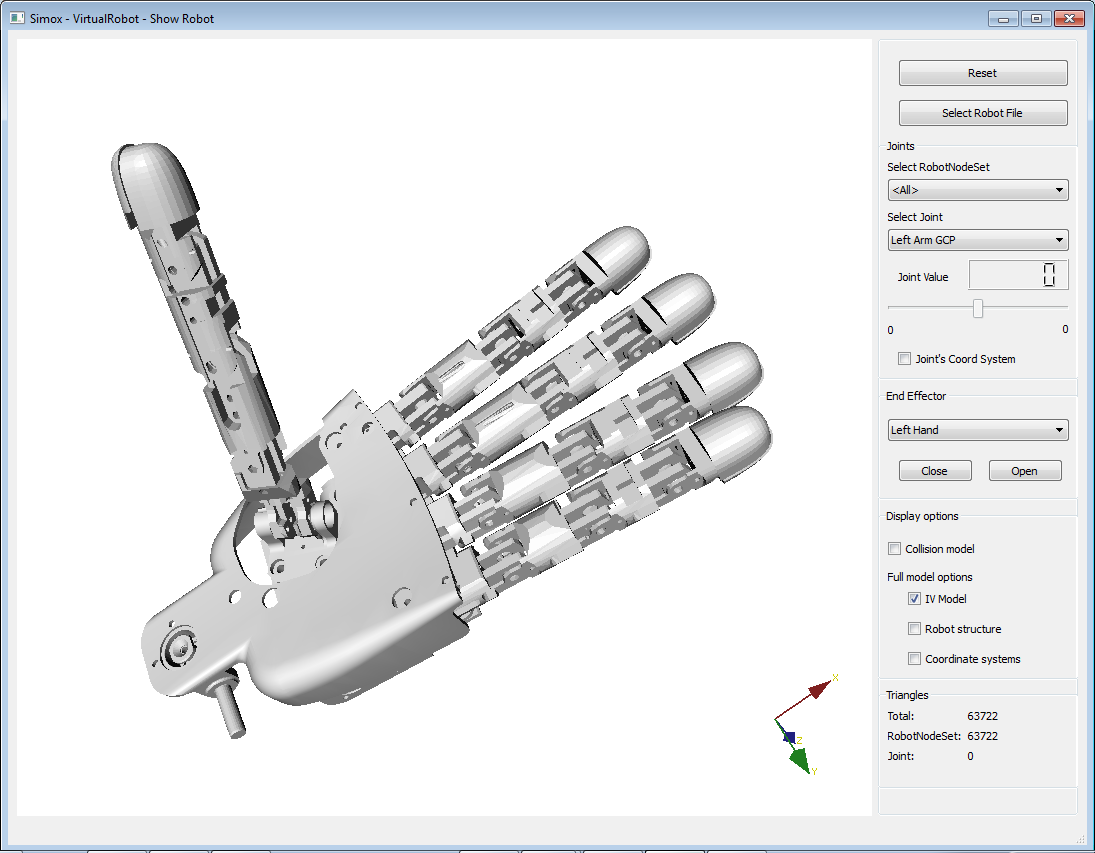
\includegraphics[width=\linewidth]{Tutorial9}
	\end{minipage}
	%\hspace{.05\linewidth}
	\begin{minipage} {.45\linewidth}
	  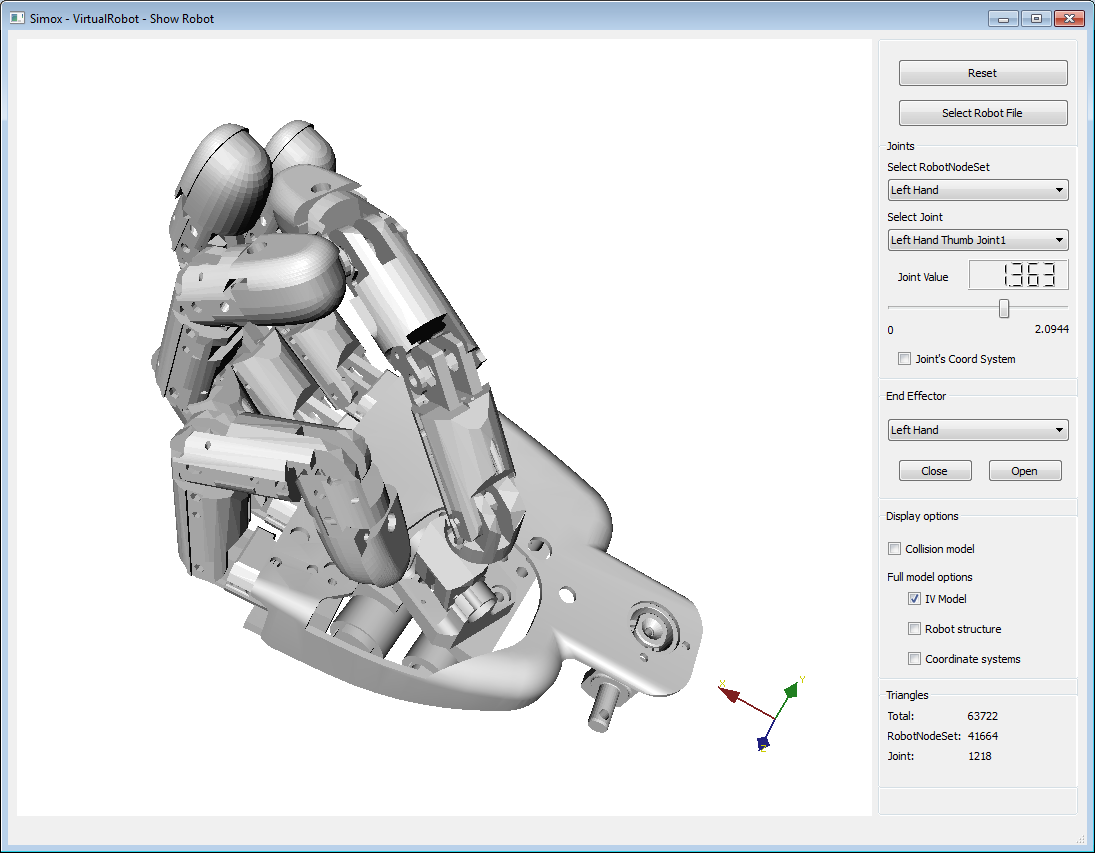
\includegraphics[width=\linewidth]{Tutorial9c}
	\end{minipage}	
\end{figure}	
\begin{figure}[H]
	\centering
	\begin{minipage} {.45\linewidth}
	  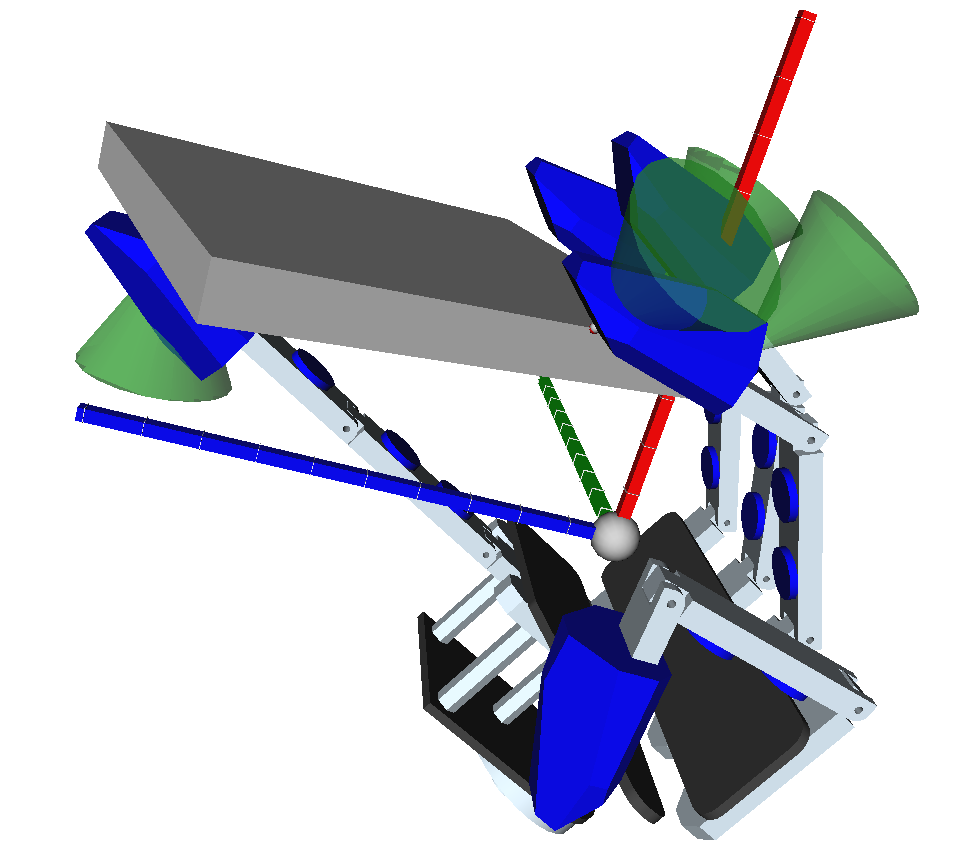
\includegraphics[width=\linewidth]{ContactPointsBox}
	\end{minipage}
\end{figure}	

\par
\subsubsection{Obstacles and Grasps}
Simple obstacles can be created as follows: 
\begin{lstlisting}
VirtualRobot::ObstaclePtr box = VirtualRobot::Obstacle::createBox(30.0f,30.0f,30.0f); // in mm
\end{lstlisting}
They can be positioned via homogeneous matrices: 
\begin{lstlisting}
box->setGlobalPose(matrix4x4);
\end{lstlisting}
Obstacles that can be grasped are called \textit{ManipulationObjects} and offer the (optional) possibility to define grasps for a specific robot/end effector. 
\begin{lstlisting}
VirtualRobot::ManipulationObjectPtr object = VirtualRobot::ObjectIO::loadManipulationObject("filename.xml");
\end{lstlisting}
The corresponding grasps can be retrieved with: 
\begin{lstlisting}
VirtualRobot::GraspSetPtr grasps = object->getGraspSet("myRobot", "myEEF");
\end{lstlisting}
A grasp can be accessed as follows: 
\begin{lstlisting}
VirtualRobot::GraspPtr g = grasps->getGrasp(0);
VirtualRobot::GraspPtr g2 = grasps->getGrasp("name of grasp");
\end{lstlisting}
\textbf{A grasp basically defines a object related pose of the end effector, whereas the pose of the end effector is given in its TCP coordinate system}.\par To get the resulting pose for the TCP, when considering the object at pose mObject, you can use the following method: 
\begin{lstlisting}
Eigen::Matrix4f mTCP = g->getTcpPoseGlobal(mObject);
\end{lstlisting}
If you want to compute the pose that an object has to be set to, in order that the grasp g can be applied, you need to pass a robot, which is used to retrieve the current configuration: 
\begin{lstlisting}
Eigen::Matrix4f mObject = g->getTargetPoseGlobal(robot);;
\end{lstlisting}
Scenes are a collection of robots, obstacles, and ManipulationObjects. A scene can be loaded and accessed in the following way: 
\begin{lstlisting}
VirtualRobot::ScenePtr scene = VirtualRobot::SceneIO:loadScene("scenefile.xml");

// access robots
std::vector<VirtualRobot::RobotPtr> robots = scene->getRobots();
VirtualRobot::RobotPtr robot = scene->getRobot("name of robot");

// get all configurations for a specific robot
 std::vector<VirtualRobot::RobotConfigPtr > configs = scene->getRobotConfigs(robot);

// get all Obstacles/ManipulationObjects
std::vector<VirtualRobot::ManipulationObjectPtr> manipObjects = scene->getManipulationObjects();
std::vector<VirtualRobot::ObstaclePtr> obstacles = scene->getObstacles();

// get sets of SceneObjects (== obstacles or manipulationobjects)
std::vector<VirtualRobot::SceneObjectSetPtr> objectSets = scene->getSceneObjectSets();
\end{lstlisting}
\begin{figure}[H]
	\centering
	\begin{minipage} {.45\linewidth}
	  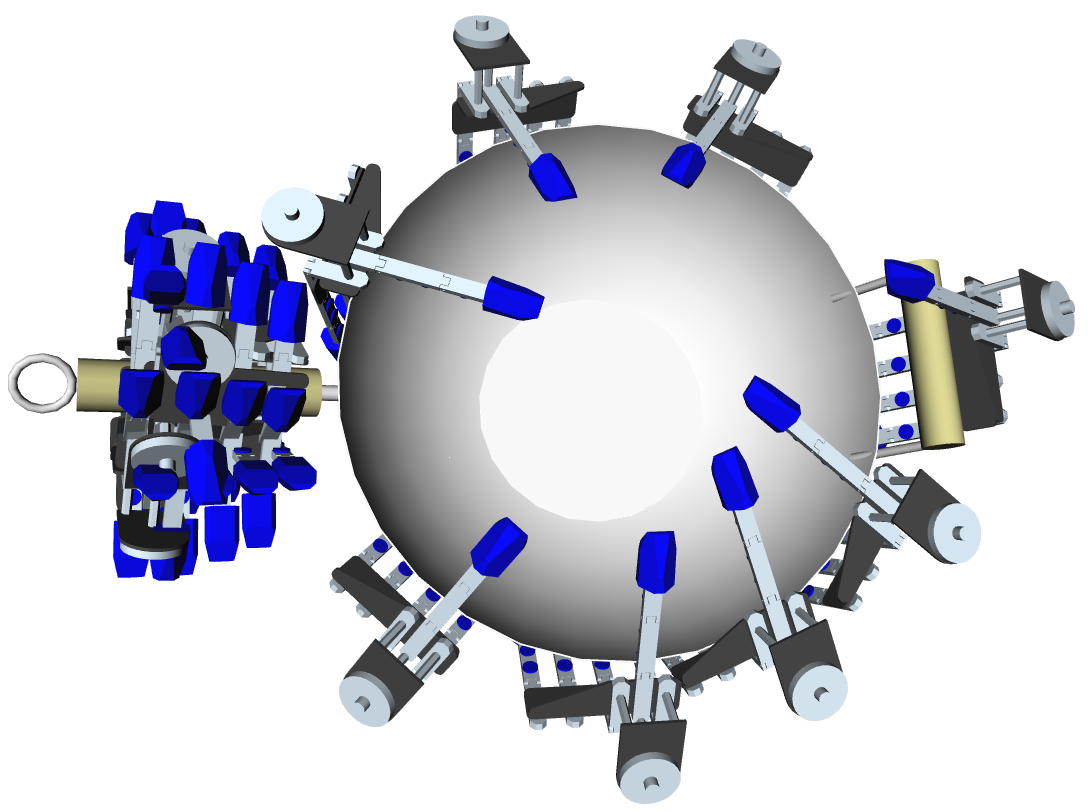
\includegraphics[width=\linewidth]{Wok_grasps_EEF}
	\end{minipage}
	%\hspace{.05\linewidth}
	\begin{minipage} {.45\linewidth}
	  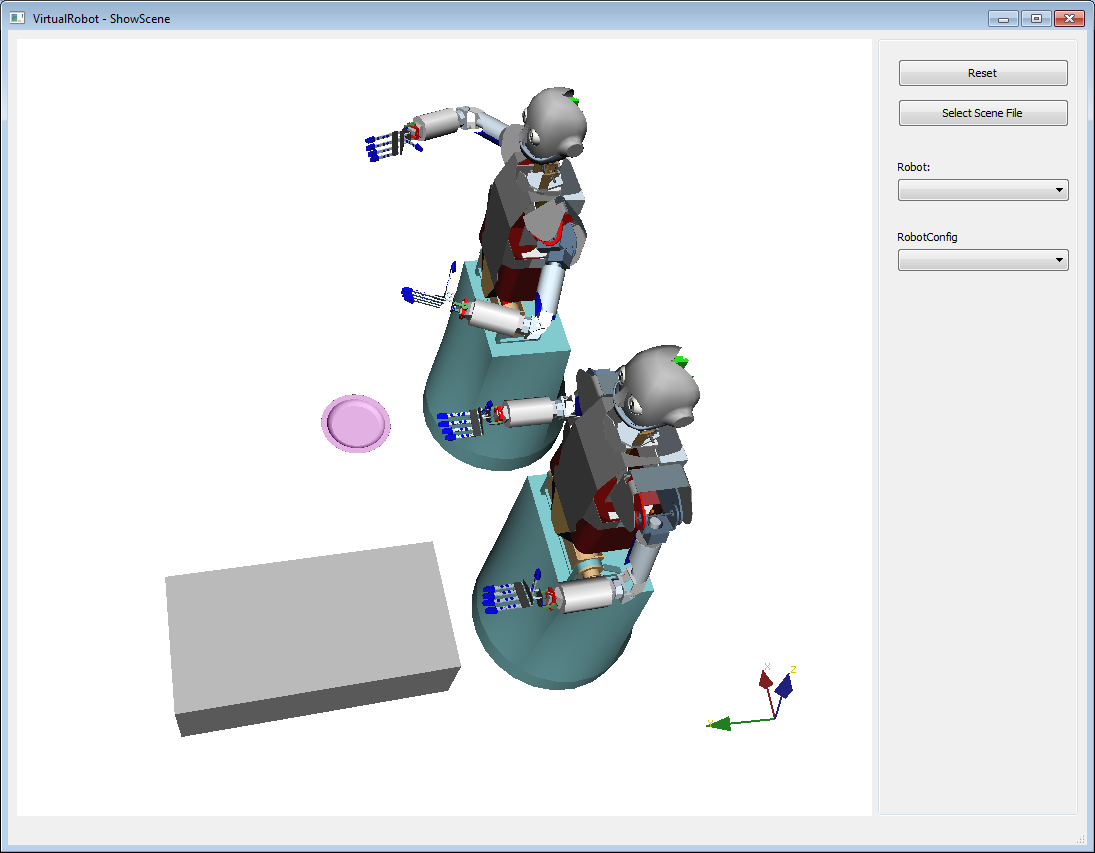
\includegraphics[width=\linewidth]{Tutorial10}
	\end{minipage}	
\end{figure}
\subsubsection{Visualization}
Depending on the cmake setup, different visualization engines can be used. Currently Coin3D is fully supported. Additionally, an exemplary implementation for OpenSceneGraph is provided, but not all visualization features are supported right now.
\subsubsection*{Open Inventor / Coin3D (recommended)}
To use Coin3D's Open Inventor API we recommend to perform a setup together with Qt and SoQt (a Coin3D library that allows to easily render OpenInventor scenes to a Qt widget).\par
For this example, we assume that you have created an Qt-UI class (e.g. with QtDesigner) that holds an empty Qt::Frame named frameViewer.\par
The following code examples are taken from the VirtualRobot example RobotViewer. 
\begin{itemize}
\item The following variables are needed to setup your environment. The Coin3D's SoSeparators are used to hold the Open Inventor data and the SoQtExaminerViewerSoQt class from the SoQt library is used to embed a Qt widget for rendering.
\begin{lstlisting}
	SoSeparator *sceneSep;
    SoSeparator *robotSep;
    boost::shared_ptr<VirtualRobot::CoinVisualization> visualization;
    SoQtExaminerViewer *viewer;
\end{lstlisting}
\item Initialization 
\begin{lstlisting}
    sceneSep = new SoSeparator;
    sceneSep->ref();
    robotSep = new SoSeparator;
    sceneSep->addChild(robotSep);
    viewer = new SoQtExaminerViewer(UI.frameViewer,"",TRUE,SoQtExaminerViewer::BUILD_POPUP);
    // the following setting is needed if you want to visualize highlighted parts of the robot
    viewer->setGLRenderAction(new SoLineHighlightRenderAction);


    // some optional parameters
    viewer->setBackgroundColor(SbColor(1.0f, 1.0f, 1.0f));
    viewer->setAccumulationBuffer(true);
    viewer->setAntialiasing(true, 4);
    viewer->setTransparencyType(SoGLRenderAction::SORTED_OBJECT_BLEND);
    viewer->setFeedbackVisibility(true);
    viewer->setSceneGraph(sceneSep);
    viewer->viewAll();
\end{lstlisting}
\item A loaded robot can be added to the visualization as follows:
 \begin{lstlisting}
    SceneObject::VisualizationType visuMode = SceneObject::Full;
    visualization = robot->getVisualization<CoinVisualization>(visuMode);
    SoNode* visualisationNode = visualisationNode = visualization->getCoinVisualization();
    robotSep->addChild(visualisationNode);
\end{lstlisting}
\end{itemize}

\subsubsection*{OpenSceneGraph}
A robot and objects can be visualized in a Qt window using the VirtualRobot::osgViewerWidget class. This widget supports OSG renderings and it can be embedded in an Qt::Frame (you can setup your window with QtDesigner and add an empty Frame that is accessed from the code).
\par
The following code examples are taken from the VirtualRobot example RobotViewerOSG. 
\begin{itemize}
\item For setting up your environment use the following variables: 
\begin{lstlisting}
    osg::Group* osgRoot;     
    osg::Group* osgRobot;
    VirtualRobot::osgViewerWidget* osgWidget;
    boost::shared_ptr<VirtualRobot::OSGVisualization> visualization;
\end{lstlisting}
\item Initialization 
\begin{lstlisting}
    osgRoot = new osg::Group();
    osgRobot = new osg::Group();
    osgRoot->addChild(osgRobot);
    osgWidget = new VirtualRobot::osgViewerWidget(osgRoot,UI.frameViewer);
    sgWidget->show();
\end{lstlisting}
\item A loaded robot can be added to the visualization as follows: 
\begin{lstlisting}
    SceneObject::VisualizationType visuMode = SceneObject::Full;
    visualization = robot->getVisualization<OSGVisualization>(visuMode);
    osg::Node* visualisationNode = visualisationNode = visualization->getOSGVisualization();
    osgRobot->addChild(visualisationNode);
\end{lstlisting}
\end{itemize}
\subsubsection{Collision Detection}
Collision Detection is a crucial part of any sampling-based motion planning algorithm. Hence, Simox takes special care of efficiently handling collision and distance queries. 
\par
\subsubsection*{Collision Engine}
\par
Simox allows to exchange the collision detection engine. By default a slightly updated version of the efficient and reliable library PQP is used. The sources are shipped with simox and the compilation process is handled by cmake, so there is no need of installing PQP on your own. An advantage of PQP is, that no prerequisites have to be met by the model representation as long as they exist as a set of triangles. PQP handles unordered sets of triangles with high efficiency.
\par
If you intend to use a different collision engine have a look at the sources in VirtualRobot/CollisionDetection. 
\par
\subsubsection*{Collision Checker}
\par
In Simox a global collision checker singleton exists that can be accessed as follows: 
\begin{lstlisting}
VirtualRobot::CollisionCheckerPtr collisionChecker = VirtualRobot::CollisionChecker::getGlobalCollisionChecker();
\end{lstlisting}
If you do not plan to implement multi-threaded collision queries, this collision checker object is all you need. 
\par
\subsubsection*{Collision Models}
All models (Objects, Obstacles, Robots, RobotNodes, etc) in Simox have two 3D representations. One for visualization (high def) and one for collision detection purposes (low def). You can visualize the models as well as the internal triangulated data structure by passing teh corresponding VirtualRobot::SceneObject::VisualizationType flag (Full, Collison, CollisionData) to the visualization routines. The collision models are usually defined in the robot's or object's XML description file. You can access them with: 
\begin{lstlisting}
VirtualRobot::CollisionModelPtr colModel = object->getCollisionModel();
\end{lstlisting}
\subsubsection*{Collision and Distance Queries}
The collision checker can be asked if two models are in collision or not:  
\begin{lstlisting}
bool inCollision = collisionChecker->checkCollision(colModel1,colModel2);
\end{lstlisting}
Additionally, the shortest distance between the two surfaces can be queried. The following code fragment shows how to get the shortest distance and the corresponding points on the object's surface: 
\begin{lstlisting}
Eigen::Vector3f surface1,surface2;
float dist = collisionChecker->calculateDistance(colModel1,colModel2,surface1,surface2);
\end{lstlisting}
Instead of using the collision models, SceneObjects (and all derived objects like Obstacles and RobotNodes) can be directly passed to the collision checker: 
\begin{lstlisting}
VirtualRobot::ObstaclePtr obstacle = VirtualRobot::Obstacle::createBox(100.0f,100.0f,100.0f);
obstacle->setGlobalPose(Eigen::matrix4f::Identity());
VirtualRobot::RobotNodePtr robotNode = robot->getRobotNode("Joint1");
bool inCollision = collisionChecker->checkCollision(robotNode,obstacle);
\end{lstlisting}
When operating with sets of objects (like kinematic chains, or a bunch of obstacles) you can use SceneObjectSets and RobotNodeSets as well: 
\begin{lstlisting}
VirtualRobot::ObstacleSetPtr obstacles = scene->getSceneObjectSet("All Obstacles");
VirtualRobot::RobotNodeSetPtr kinChain = robot->getRobotNodeSet("Left Arm");
float minDist = collisionChecker->calculateDistance(kinChain,obstacles);
\end{lstlisting}
\subsubsection*{Complex Collision Setups}
Complex collision queries can be handled with the VirtualRobot::CDManager class. Here multiple pairs of object(s) can be specified which all should be checked for validity. This can be useful when multiple parts of a robot have to be considered, e.g. for motion planning.
\par
In the following example an obstacle and a robot node are selected for collision detection. Additionally any self collisions between the kinematic structures of the arm and the torso and head should be considered.  
\begin{lstlisting}
VirtualRobot::CDManagerPtr cdm(new VirtualRobot::CDManager());
cdm->addCollisionPair(obstacle,robotNode);
cdm->addCollisionPair(rnsArm,rnsTorso);
cdm->addCollisionPair(rnsArm,rnsHead);
bool inCollision = cdm->isInCollision();
\end{lstlisting}
\subsubsection{Workspace Analysis: Reachability and Manipulability}
 A representation of the spatial reachability of a robot's manipulator can be precomputed in order to efficiently search for reachable grasps/poses during online processing. To this end a 6D voxel grid is filled, either with binary values (reachable/not reachable) or with quality information that indicates how well a pose can be reached. E.g. the manipulability can be used as such a quality measure.
\par
From the base class for performing workspace analysis WorkspaceRepresentation, currently two derivations exist: 
\begin{itemize}
\item Reachability: This implementation can be used to encode reachable 6D poses with a simple quality measure which is related to the volume in joint space that maps to a voxel.
\begin{itemize}
\item Creation \par
Assuming a robot and a RobotNodeSet rns exist, an empty instance of the reachability can be created as follows:
\begin{lstlisting}
  ReachabilityPtr reachSpace(new Reachability(robot));
        reachSpace->initialize(rns,discrTr,discrRo,minB,maxB,staticModel,dynamicModel,baseNode,tcpNode);
        reachSpace->print();
\end{lstlisting}
\item Filling with data and IO  \par
 The reachability representation is initialized with two discretization parameters: discrTrans, the voxel size in translational components and discrRot, teh discretization for the three rotational dimensions. Further, the bounding box and in case self-collisions should be considered, a setup for collision detection is passed.\par
 The reachability data can be filled by adding randomly generated robot poses (e.g. 1 mio poses): 
 \begin{lstlisting}
        reachSpace->addRandomTCPPoses(1000000);
        reachSpace->print();
        reachSpace->save("myReachFile.bin");
        reachSpace.reset(new Reachability(robot));
        reachSpace->load("myReachFile.bin");
        reachSpace->print();
 \end{lstlisting}
 \item Querying  \par
   The reachability data can be queried extremely fast. Here is an example: 
    \begin{lstlisting}
        // get all grasps that are reachable
        ManipulationObjectPtr object; // an object
        // load object ....
        GraspSetPtr reachableGrasps = reachSpace->getReachableGrasps(allGrasps, object); 
    \end{lstlisting}
     \item Demo  \par
     A reference implementation of reachability analysis can be found in VirtualRobot's example directory. The `ReachabilityDemo` can be used to build and visualize reachability data for custom robots and manipulators. The tool can be used to show myRobot.xml with a custom reachability file myReachFile.xml and by specifying the main TCP direction for visualization purposes. 
     \end{itemize} 
     \begin{lstlisting}
    ReachabilityDemo --robot myRobot.xml --reachability myReachFile.bin --visualizationTCPAxis (1,0,0) 
        \end{lstlisting} 
 
\item Manipulability: This class encapsulates an enhanced workspace representation that uses a basic manipulability measure for determining the quality of robot poses. Custom implementations of quality measures can be used as well.  
\begin{itemize}
\item Here is a short example: 
     \begin{lstlisting}
        ManipulabilityPtr manipulability(new Manipulability(robot));
        PoseQualityManipulabilityPtr measure(new PoseQualityManipulability(rns)); // basic manipulability measure
        measure->penalizeJointLimits(true,50000); // penalize poses near joint limits
        manipulability->setManipulabilityMeasure(measure);
        float minB[6];
        float maxB[6];
        float maxManip;
        // automatically determine parameters
        manipulability->checkForParameters(rns,2000,minB,maxB,maxManip,baseNode,tcpNode);
        manipulability->initialize(rns,discrTr,discrRo,minB,maxB,staticModel,dynamicModel,baseNode,tcpNode);
        manipulability->setMaxManipulability(maxManip);
        manipulability->print();  
        \end{lstlisting}
\item Data and hole filling 
Add some random configs and smooth the result: 
     \begin{lstlisting}
        manipulability->addRandomTCPPoses(steps);
        manipulability->smooth(2);
        manipulability->print();  
        \end{lstlisting}
\end{itemize}
\item Reachability Maps are useful to determine promising robot base positions for grasping. Based on a reachability distribution of the manipulator, the reachability map can becomputed as a discretized 2D distribution serving potential robot positions for reaching a grasping pose. 
\begin{lstlisting}
    // get boundong box extends of manipulator's reachability 
    Eigen::Vector3f minBB,maxBB;
    reachSpace->getWorkspaceExtends(minBB,maxBB);
    // build reachability grid in x/y plane with identical discretization
    WorkspaceGridPtr reachGrid(new WorkspaceGrid(minBB(0),maxBB(0),minBB(1),maxBB(1),reachSpace->getDiscretizeParameterTranslation()));

    // the target object 
    ManipulationObjectPtr graspObject = ObjectIO::loadManipulationObject("myObject.xml");
    // and a specific grasp
    GraspPtr g = graspObject->getGrasp("myGrasp1");

    // position the reachability grid
    Eigen::Matrix4f gp = graspObject->getGlobalPose();
    reachGrid->setGridPosition(gp(0,3),gp(1,3));

    // fill the grid according to one specific grasp
    reachGrid->fillGridData(reachSpace, graspObject, g, robot->getRootNode() );


    // or: fill the grid with all grasps
    EndEffectorPtr eef = robot->getEndEffector("Right Hand");
    GraspSetPtr grasps = graspObject->getGraspSet(eef);
    for (int i=0;i<(int)grasps->getSize();i++)
    {
        g = grasps->getGrasp(i);
        reachGrid->fillGridData(reachSpace, graspObject, g, robot->getRootNode() );
    }

    // sample a base pose with minimum quality of 1
    // the result is stroed in x,y together with the corresponding grasp g
    float x,y;
    bool ok = reachGrid->getRandomPos(1, x, y, g,);
\end{lstlisting}
The `ReachabilityMap` tool can be used to examine the behavior of this approach.\par
\begin{figure}[H]
	\centering
	\begin{minipage} {.45\linewidth}
	  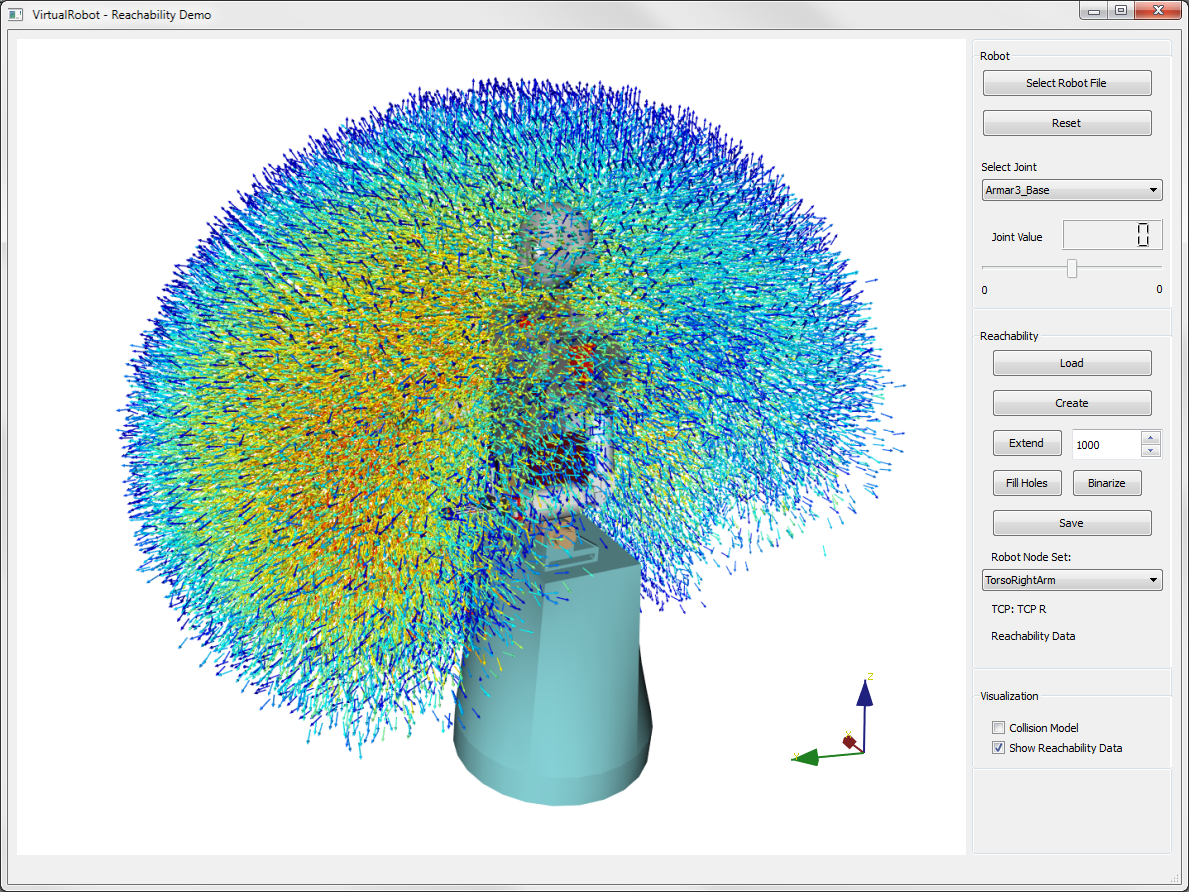
\includegraphics[width=\linewidth]{Reachability_HipRightArm_ArmarIII}
	\end{minipage}
	%\hspace{.05\linewidth}
	\begin{minipage} {.45\linewidth}
	  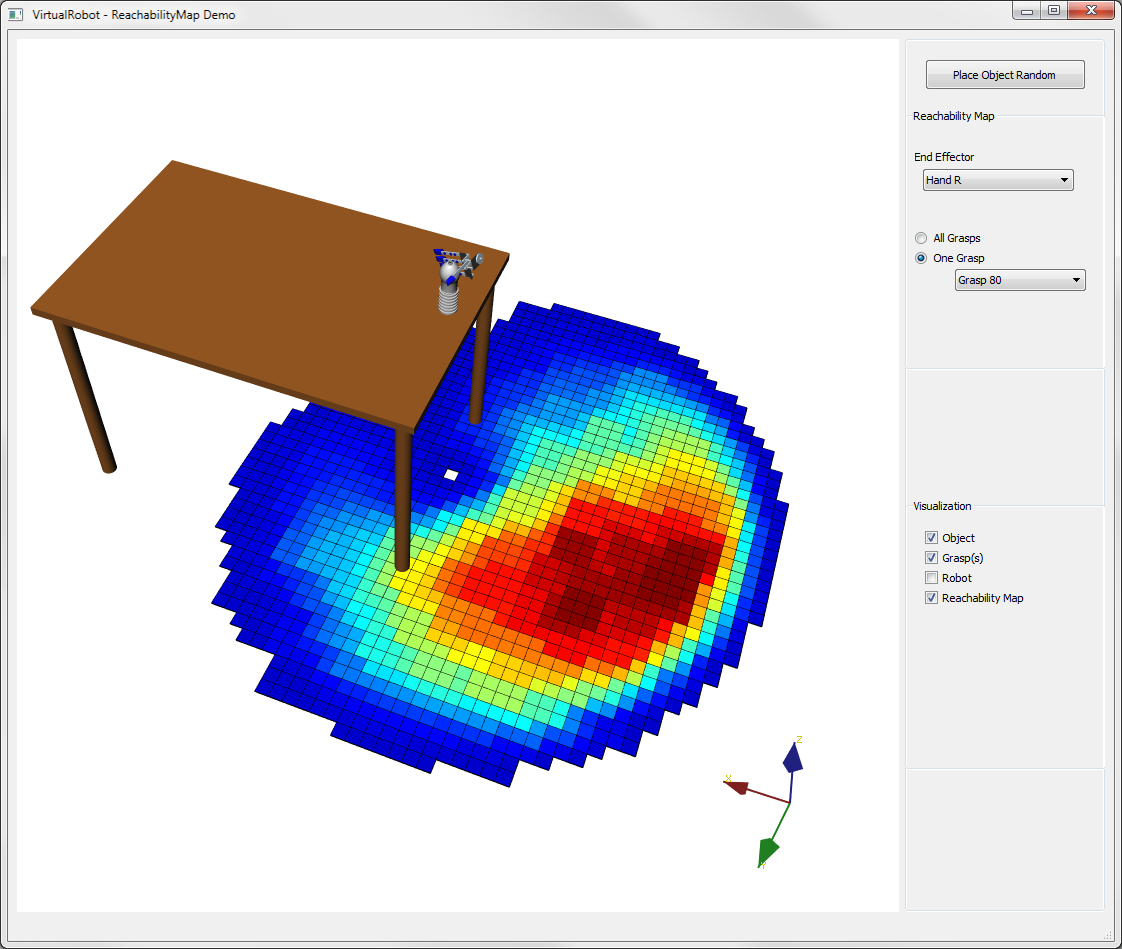
\includegraphics[width=\linewidth]{Reachmap}
	\end{minipage}
\end{figure}
\begin{figure}[H]
	\centering
	\begin{minipage} {.45\linewidth}
	  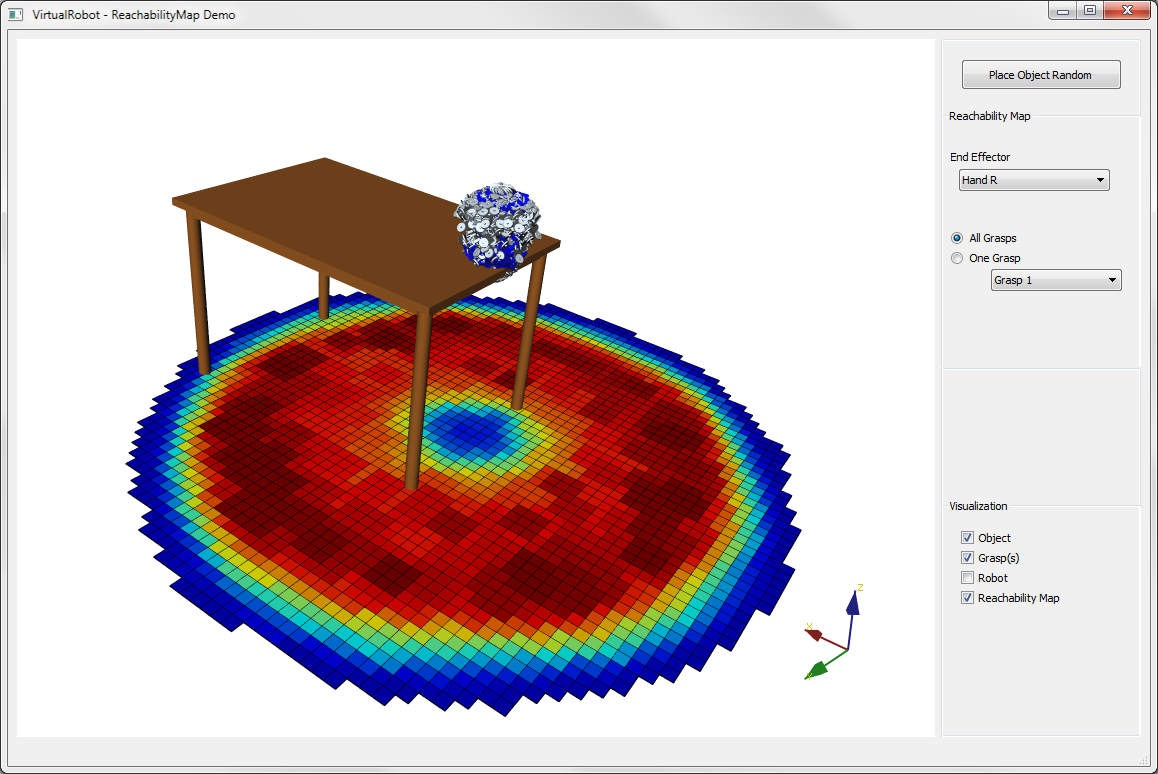
\includegraphics[width=\linewidth]{ReachMapAll}
	\end{minipage}
	%\hspace{.05\linewidth}
\end{figure}
\end{itemize}
\subsubsection{Jacobians and IK solving}
Simox provides a generic IK solver, which is based on the Jacobian's Pseudoinverse approach. The IK solver is instantiated with a kinematic chain and it can be queired for 3D or 6D poses. The GenericIKDemo and JacobiDemo provide exemplary implementations. Here is a short example:
\begin{lstlisting}
RobotNodeSetPtr kc = robot->getRobotNodeSet("Left Arm");
// several Jacobi inversions algorithms are available
// here, the SVD damped approach is used
GenericIKSolverPtr ikSolver(new GenericIKSolver(kc, JacobiProvider::eSVDDamped));

// solve a query (only position)
Eigen::Matrix4f pose = kc->getTCP()->getGlobalPose();
pose(0,3) += 10.0f; // move 10 mm
bool ok = ikSolver->solve(pose,IKSolver::Position);

// solve a query (position and orientation)
// setup stepsize and max gradient decent loops
// lower stepsize -> better convergence but slower
// max loops: Just needed in special cases. Internally the iterative process is
// canceled when no progress has been made in the last step
ikSolver->setupJacobian(0.3f, 30); 
ok = ikSolver->solve(pose,IKSolver::All);

// Search solution to one of the grasps of the ManipulationObject
// current pose of object is considered
ok = ikSolver->solve(object, IKSolver::All);

// Search solution for one specific grasp applied to the object
GraspPtr g = object->getGraspSet("LeftHand")->getGrasp("Grasp0");
ok = ikSolver->solve(object, g, IKSolver::All);

// By default, the current configuration of the robot is used as start pose
// If that failes (e.g. for large distances), the IKSolver can generate random seed poses
// for the iterative gradient decent approach (50 in the following example).
ok = ikSolver->solve(pose, IKSolver::Position, 50);
\end{lstlisting}
Another example, showing how to access the Jacobians:
\begin{lstlisting}
// Setup
RobotNodeSetPtr rns = robot->getRobotNodeSet("LeftArm");
DifferentialIKPtr j(new DifferentialIK(rns));

// setup a tcp with goal
RobotNodePtr tcp = rns->getTcp();
j->setGoal(targetPose,tcp,IKSolver::Position);

// get the Jacobian matrix for the tcp setup
Eigen::MatrixXf jac = j->getJacobianMatrix();

// get the pseudoinverse
Eigen::MatrixXf jacI = j->getPseudoInverseJacobianMatrix(tcp, IKSolver::All);
\end{lstlisting}
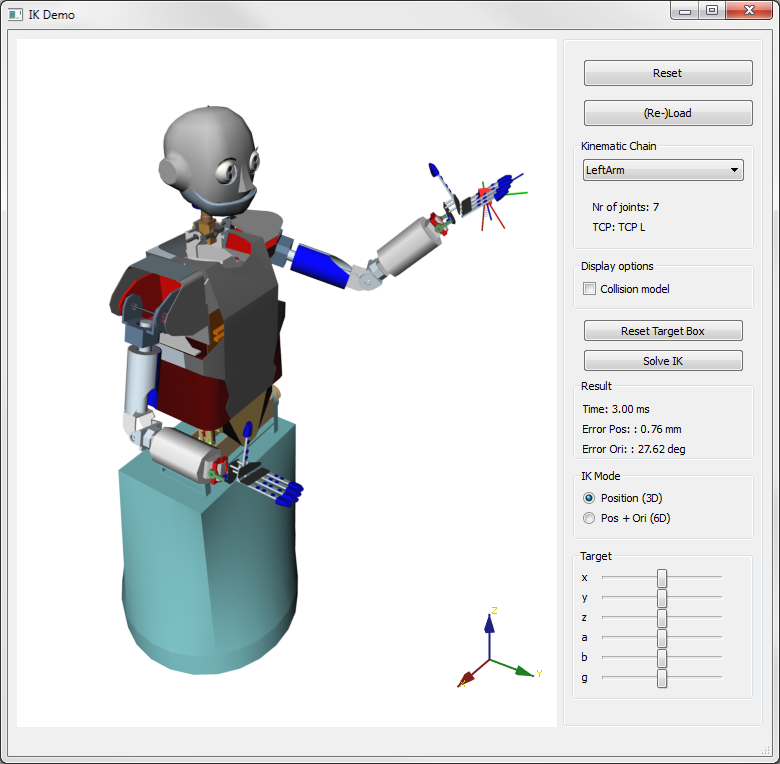
\includegraphics[width=\textwidth]{IKDemo}
\subsubsection{Hierarchical IK solving}
Complex robot systems usually have to meet multiple objectives for IK solving. Such objectives could include stability, feet postures, eef positions, etc. Simox provides methods for hierarchical IK solving, where a stack of tasks is processed by solving each task in the Null Space of the preceding tasks. Therefore JoacobiProviders are implemented for several objectives like pose reaching and stability. The framework is extendable and allows to implement custom JacobiProvides in order to combine them for hierarchical IK solving.
\begin{lstlisting}
HierarchicalIKPtr hik(new HierarchicalIK(rnsJointsAll));
std::vector<HierarchicalIK::JacobiDefinition> jacobies;

// first Right feet pose
DifferentialIKPtr ikLeft2Right(new DifferentialIK(rnsJointsAll));
Eigen::Matrix4f trafoLeft2Right = feetPosture->getTransformationLeftToRightFoot();
Eigen::Matrix4f goalRight = feetPosture->getLeftTCP()->getGlobalPose() * trafoLeft2Right;
ikLeft2Right->setGoal(goalRight,feetPosture->getRightTCP());
HierarchicalIK::JacobiDefinition jd;
jd.jacProvider = ikLeft2Right;
jacobies.push_back(jd);

// second: COM
CoMIKPtr comIK(new CoMIK(rnsJointsAll,rnsModelsAll));
supportPolygon->updateSupportPolygon(10.0f);
Eigen::Vector2f c = MathTools::getConvexHullCenter(supportPolygon->getSupportPolygon2D());
comIK->setGoal(c); 
HierarchicalIK::JacobiDefinition jd2;
jd2.jacProvider = comIK;
jacobies.push_back(jd2);

// third: EEF pose
Eigen::Matrix4f goal = tcpGoal;
DifferentialIKPtr ikTCP(new DifferentialIK(rnsJointsAll));
ikTCP->setGoal(goal,tcp);
HierarchicalIK::JacobiDefinition jd3;
jd3.jacProvider = ikTCP;
jacobies.push_back(jd3);

//compute step
Eigen::VectorXf delta = hik->computeStep(jacobies,stepsize);
Eigen::VectorXf jv(delta.rows());
rnsJointsAll->getJointValues(jv);
jv += delta;
rnsJointsAll->setJointValues(jv);
\end{lstlisting}
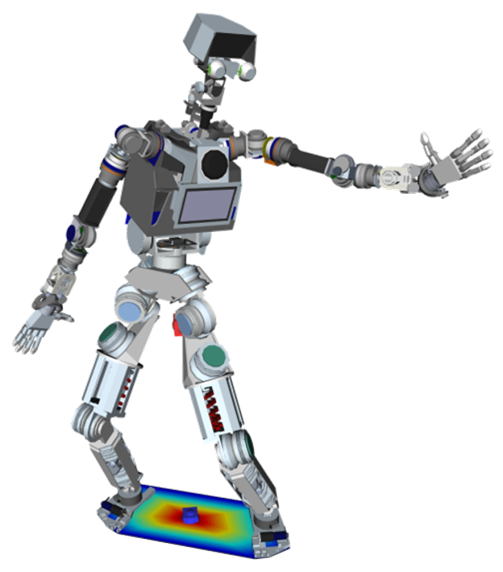
\includegraphics[width=\textwidth]{HierarchicalIK}
\subsubsection{Stability computations}
The StabilityDemo shows an exemplary usage of stability related methods.\par

The center of mass of a robot (or a RobotNodeSet) can be queried as follows: 
\begin{lstlisting}
// get com of robot
Eigen::Vector3f com = robot->getCoMGlobal();
\end{lstlisting}
The support polygon is defined by the convex hull of all contact points with the floor plane. The robot is in a statically stable pose if the projection of its center of mass (COM) on the floor lies within the support polygon. It can be computed by detecting points of the feet which are near the floor, project them to the floor plane and compute their convex hull.
\begin{lstlisting}
// Support polygon
MathTools::Plane floor =  MathTools::getFloorPlane();
std::vector< CollisionModelPtr > colModels =  
    robot->getCollisionModels();
CollisionCheckerPtr colChecker = CollisionChecker::getGlobalCollisionChecker();
std::vector< CollisionModelPtr >::iterator i = colModels.begin();
std::vector< MathTools::ContactPoint > points;
for (;i!=colModels.end();i++)
    colChecker->getContacts(floor, *i, points, 5.0f);
std::vector< Eigen::Vector2f > points2D;
for (size_t u=0;u<points.size();u++)
{
    Eigen::Vector2f pt2d = 
        MathTools::projectPointToPlane2D(points[u].p,floor);
    points2D.push_back(pt2d);
}
MathTools::ConvexHull2DPtr cv = MathTools::createConvexHull2D(points2D);

The ComIK solver allows to define a workspace target (2D) on the floor.
// comIK
CoMIK comIK(rnsJoints,rnsBodies);
comIK.setGoal(CoMTarget);
comIK.solveIK(0.3f,0,20);
\end{lstlisting}
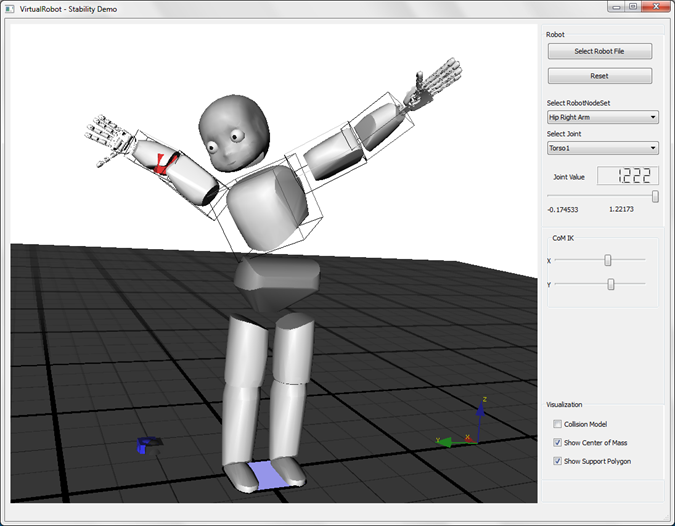
\includegraphics[width=\textwidth]{StabilityDemo}
\subsection{File formats}
\subsubsection{XSD Schema defintion}
Simox provides an XSD Schema defintion file that can be used to validate XML defintions and/or for documentation purposes. The file can be found in $<$Your\_Simox\_Dir>/doc/file\_formats.
\par
Note, that XSD definitions are case sensitive, while Simox does not consider the case while parsing XML tags. So the tags <RobotNode>, <robotnode> and <ROBOTNODE> are all starting a valid RobotNode definition. 
\subsubsection*{Types}
The following types are used: 
\begin{itemize}
\item xs:string 
\item xs:decimal
\item xs:boolean 
\item Unit-Length-Type: A string that could be "m", "meter", "mm" or "millimeter"
\item Unit-Angle-Type: A string that could be "rad", "radian", "deg" or "degree"
\item Unit-Weight-Type: A string that could be "g", "gram", "kg", "kilogram", "t" or "ton"
\item Unit-Time-Type: A string that could be "sec", "second", "min", "minute", "h" or "hour"
\item FileLocation-Type: A string that is either "absolute" or "relative", specifying whether a filename is given absolutely or relatively to the current XML file. 
\end{itemize}
\subsubsection*{Transformations}
Geometric transformations can be specified in several ways, which are encapsulated by a <Transform-Type>. Note, that either a Matrix4x4 or a rotation (Quaternion, Matrix3x3 or RollPitchYaw) together with a Translation can be used. 
\begin{itemize}
\item Matrix4x4-Type. A homogeneous transformation given as a 4x4 matrix. Here is an example:
\begin{lstlisting}
    <matrix4x4>
      <row1 c1="1" c2="0"  c3="0" c4="100"/>
      <row2 c1="0" c2="0"  c3="1" c4="200"/>
      <row3 c1="0" c2="-1" c3="0" c4="300"/>
      <row4 c1="0" c2="0"  c3="0" c4="1"/>
    </matrix4x4>
\end{lstlisting}
\item Matrix3x3-Type. A rotation given as a 3x3 matrix. Here is an example: 
\begin{lstlisting}
    <matrix3x3>
      <row1 c1="1" c2="0"  c3="0"/>
      <row2 c1="0" c2="0"  c3="1"/>
      <row3 c1="0" c2="-1" c3="0"/>
    </matrix3x3>
\end{lstlisting}
\item RollPitchYaw-Type. A rotation given as roll, pitch and yaw angles. Here is an example: 
\begin{lstlisting}
    <rollpitchyaw roll="90" pitch="0" yaw="45" unitsAngle="degree"/>
\end{lstlisting}
\item Quaternion-Type. A rotation given as quaternions. Here is an example: 
\begin{lstlisting}
    <quaternion x="1.0" y="0" z="0" w="0.2"/>
\end{lstlisting}
\item Translation-Type. A translation. Here is an example: 
\begin{lstlisting}
 <Translation x="100" y="200" z="300" unitsLength="mm"/>
\end{lstlisting}
\end{itemize}
\subsubsection{Robot Definitions}
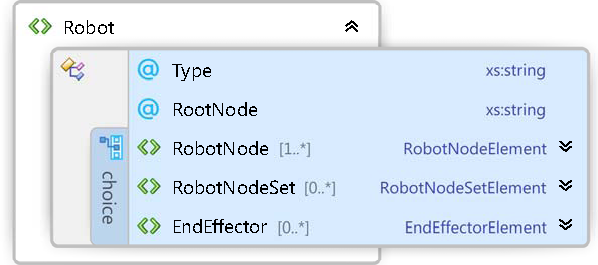
\includegraphics[width=\textwidth]{Xsd_Robot}
\subsubsection*{RobotNode}
A RobotNode can specify
\begin{itemize}
\item A fixed Transformation (optional <Transform> tag). 
\item A joint that applies a second transformation according to the joint value (optional <Joint> tag). 
\item A visualization that is linked at the resulting pose (optional <Visualization> tag). 
\item A collision model which is used for collision detection (optional <CollisionModel> tag). 
\end{itemize}
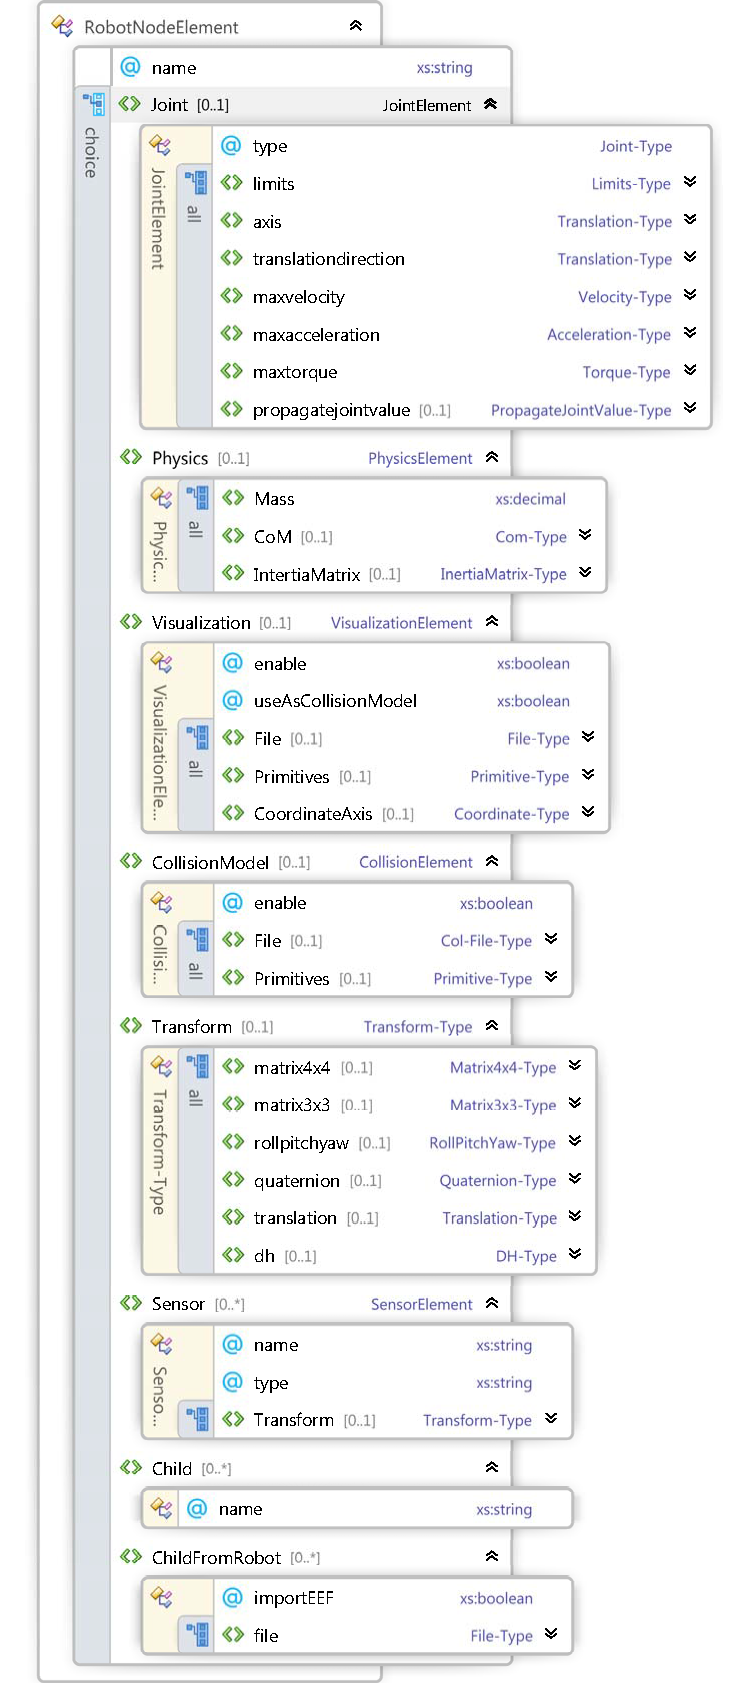
\includegraphics[width=\textwidth]{Xsd_RobotNode2}
\subsubsection*{Joint}
For each Joint tag the type has to be specified: Currently the following Joint-types are implemented:
\begin{itemize}
\item fixed (standard): A fixed joint that cannot be moved. This joint type is implicitly chosen when no joint is specified within a RobotNode.
\item  revolute: A revolute joint that can be rotated around an axis.
\item prismatic: A prismatic joint that realizes a translational movement. 
\end{itemize}
As shown below, Joints can be defined either with Denavit-Hartenberg conventions (<DH>), or by defining transformations (<Axis> or <TranslationDirection>). A valid Joint definition must either be defined the first or the second way; mixing is not allowed and will result in an exception during parsing.
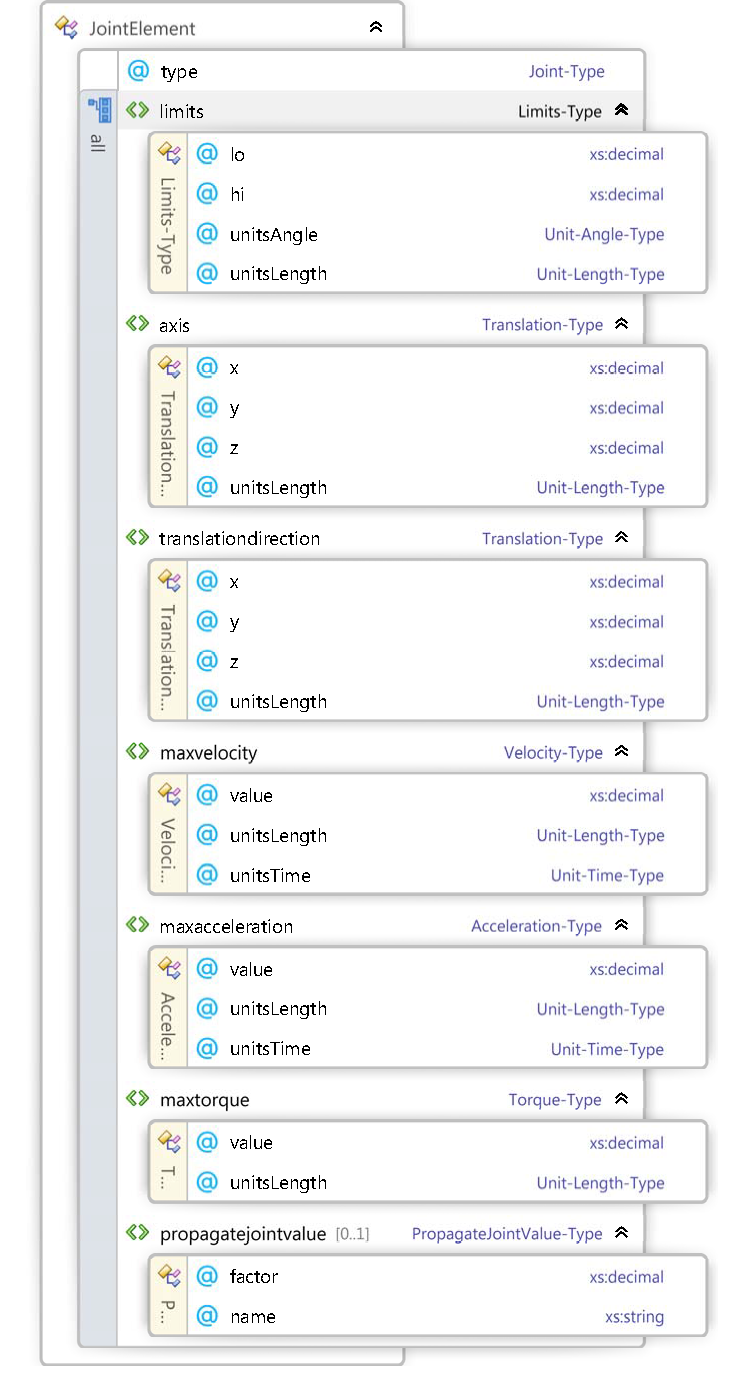
\includegraphics[width=\textwidth]{Xsd_Joint2}    

\subsubsection*{Physics}
The Coord-Location-type is a string that specifies where the CoM is located. When it's set to "VisualizationBBoxCenter" the CoM location is automatically set to the center of the bounding box of the RobotNode's visualization and the other attributes are ignored. If set to "joint", the CoM location is defined by the x,y,z attributes in the joint's coordinate system. 
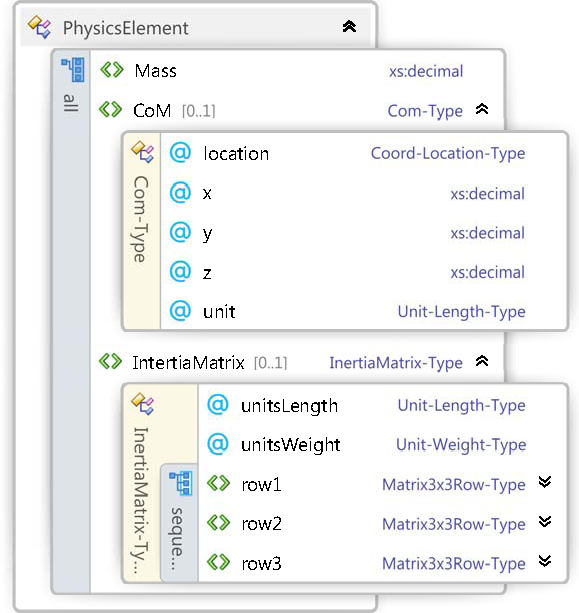
\includegraphics[width=\textwidth]{Xsd_Physics} 
\subsubsection*{Visualization}
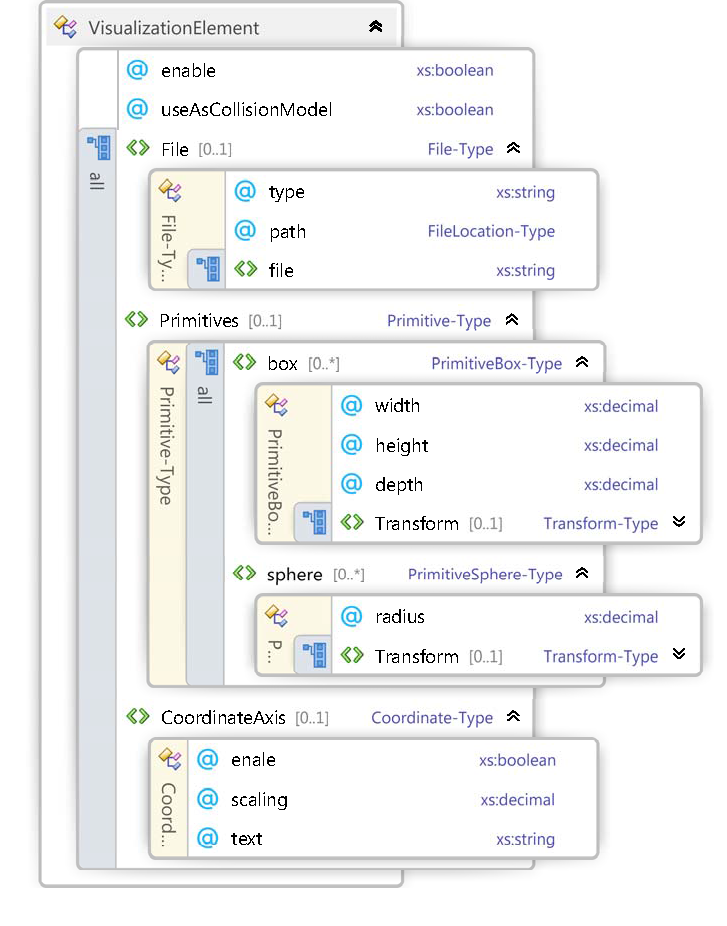
\includegraphics[width=\textwidth]{Visualization} 
Here is an example:
\begin{lstlisting}
<ManipulationObject name='MyObject'>
        <Visualization>
            <Primitives>
                <Box width="136" height="190" depth="40"/> <!-- primitive-specific parameters, default unit is mm -->
                <Sphere radius="0.15" unitslength="m">
                    <Transform> <!-- transform is relative to previous primitive -->
                        <Translation x="0" y="170" z="0"/>
                    </Transform>
                </Sphere>
                <Box width="136" height="190" depth="40">
                    <Transform> <!-- transform is relative to previous primitive -->
                        <Translation x="0" y="-355" z="0"/>
                        <rpy roll="0" pitch="1.41" yaw="0" unitsAngle="radian"/>
                    </Transform>
                </Box>
                <!-- other primitives -->
            </Primitives>
            <UseAsCollisionModel/>
        </Visualization>
    </ManipulationObject>
\end{lstlisting}
\subsubsection*{CollisionModel}
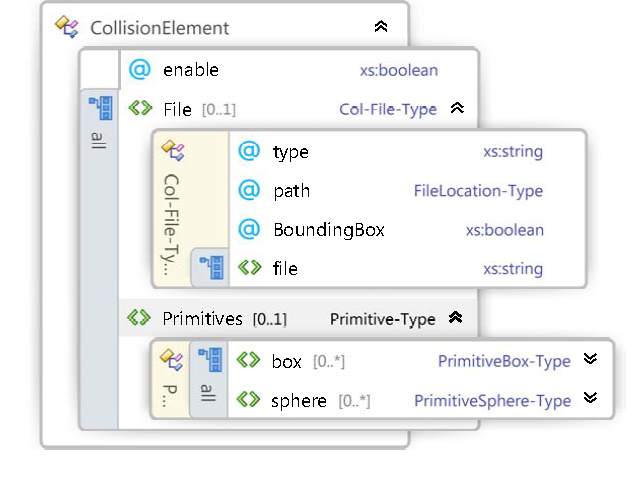
\includegraphics[width=\textwidth]{Xsd_CollisionModel} 
\subsubsection*{Sensor}
Sensors are located w.r.t. the coordinate system of the RobotNode and can additionally define a local transformation. Currently two types of sensors are implemented: Position and Camera. 
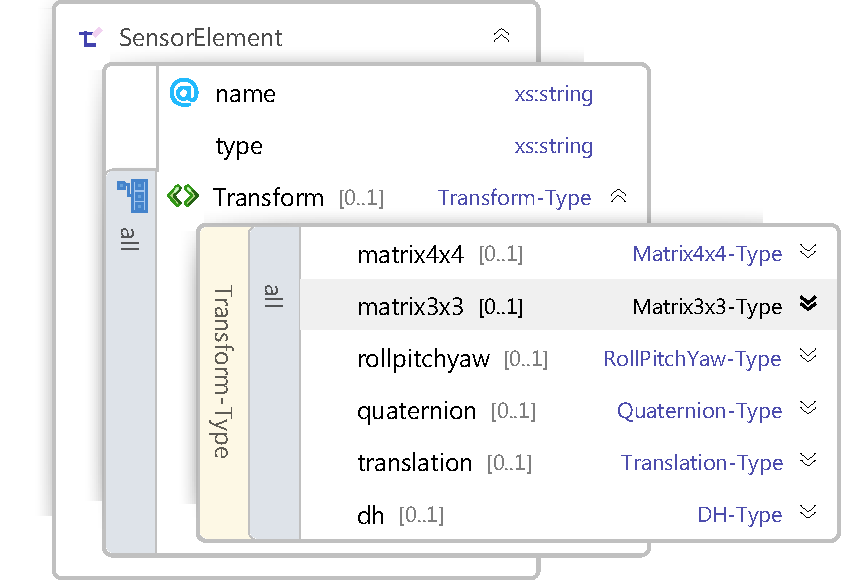
\includegraphics[width=\textwidth]{Xsd_Sensor} 
\subsubsection*{RobotNodeSet}
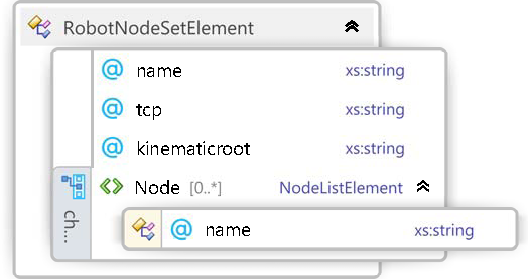
\includegraphics[width=\textwidth]{Xsd_RobotNodeSet} 
\subsubsection*{EndEffector}
The EEFActorCollision-Type specifies if and how the element of an finger/actor should be considered for collision detection. The string attribute can be 
\begin{itemize}
\item None: No collision detection should be performed with this segment. 
\item Actors: Collision detection is performed with all other actors. 
\item Static: Collision detection is performed with the static part of the EEF. 
\item All: Collision detection is performed with all other actors and the static part. 
\end{itemize}
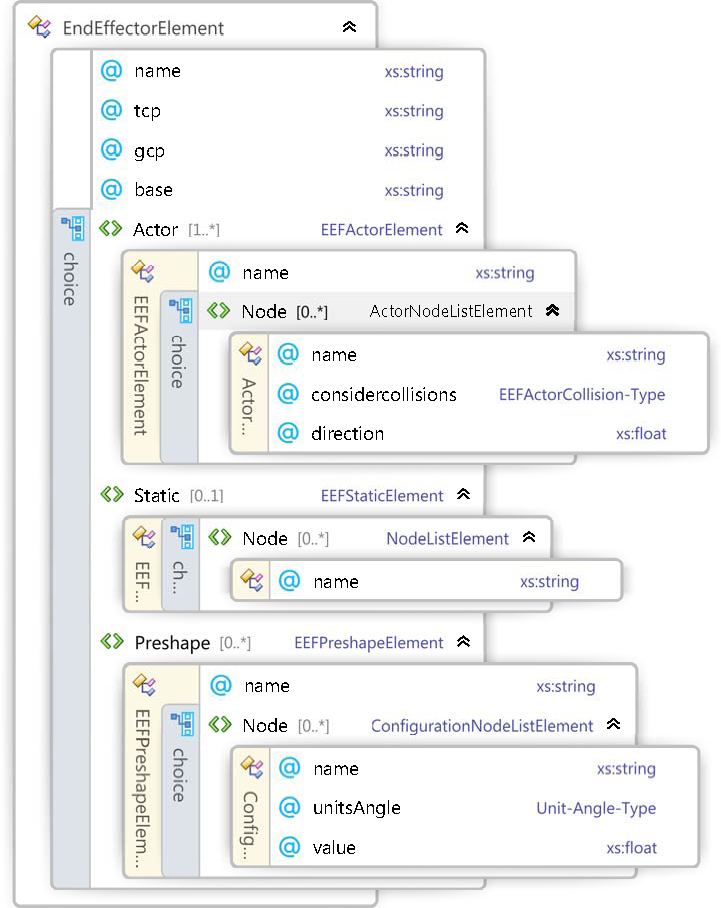
\includegraphics[width=\textwidth]{Xsd_EEF_open} 
\subsubsection{Obstacles and Manipulation Objects}
Obstacles are defined in the following way
\begin{lstlisting}
    <Obstacle name='MyObstacle'>
        <Visualization>
            <File type='inventor'>obstacleHD.iv</File>
        </Visualization>
        <CollisionModel>
            <File type='inventor'>obstacleLD.iv</File>
        </CollisionModel>
    </Obstacle>
\end{lstlisting}
In addition you can add a physics tag (see above for details) and you can specify a pose in the world via the GlobalPose tag (an example is given below).
\par
ManipulationObjects are Obstacles with additional grasping information. Note that grasping information is usually built with tools (see e.g. the Simox tools GraspEditor or GraspPlanner).
\par
Here is an example:
\begin{lstlisting}
<ManipulationObject name='MyGraspableObject'>
        <Visualization>
            <File type='inventor'>obstacleHD.iv</File>
            <UseAsCollisionModel/>
        </Visualization>
        <Physics>
                <Mass unit='kg' value='1.5'/>
                <CoM location='VisualizationBBoxCenter'/>
        </Physics>
        <GraspSet name='GraspSet LeftHand' RobotType='iCub' EndEffector='Left Hand'>
            <Grasp name='Left Grasp0' quality='1' Creation='Manual'>
                <Transform>
                    <Matrix4x4>
                        <row1 c1='0.405401' c2='-0.804495' c3='-0.434087' c4='175.361'/>
                        <row2 c1='0.908675' c2='0.406443' c3='0.0953756' c4='-28.2655'/>
                        <row3 c1='0.0997043' c2='-0.433115' c3='0.895803' c4='49.7284'/>
                        <row4 c1='0' c2='0' c3='0' c4='0.999997'/>
                    </Matrix4x4>
                </Transform>
            </Grasp>
        </GraspSet>
    </ManipulationObject>
\end{lstlisting}
You can examine Objects and ManipulationObjects directly with the Simox tool SimoxSceneViewer.
\subsubsection{Scenes}
Scenes are specified in the Simox scene file format, which is a straight forward definition of an environment consisting of robot(s) and/or obstacles. You can link to existing Robot/Obstacle/ManipulationObject files and you are allowed to add further information.
\par
The following example shows 
\begin{itemize}
\item how to add a robot to the scene, how to define the location of the robot, and how to define configurations which can be accessed via the API.
\item how to add obstacles by directly referring to 3D mesh files
\item how to include existing Obstacle/ManipulationObject files
\end{itemize}
\begin{lstlisting}
<Scene name="iCubScene">
    <Robot name="iCub">
        <File>robots/iCub/iCub.xml</File>
        <Configuration name="start">
            <Node name="Shoulder 1 L" unit="radian" value="-0.85"/>
            <Node name="Shoulder 2 L" unit="radian" value="-0.8"/>
            <Node name="Upperarm L" unit="radian" value="-0.85"/>
            <Node name="Shoulder 1 R" unit="radian" value="-0.85"/>
            <Node name="Shoulder 2 R" unit="radian" value="0.8"/>
            <Node name="Upperarm R" unit="radian" value="0.85"/>
        </Configuration>
        <GlobalPose>
            <Transform>
                <Translation x="9000" y="1500" z="500"/>
                <rollpitchyaw units="degree" roll="0" pitch="0" yaw="180"/>
            </Transform>
        </GlobalPose>
    </Robot>

    <Obstacle name="Box">
        <Visualization>
            <File type="Inventor" path="relative">../objects/iv/box1000x500x300.iv</File>
            <UseAsCollisionModel/>
        </Visualization>
        <GlobalPose>
            <Transform>
                <Translation x="9000" y="1500" z="150"/>
                <rollpitchyaw units="degree" roll="0" pitch="0" yaw="90"/>
            </Transform>
        </GlobalPose>
    </Obstacle>

    <ManipulationObject name="RiceFit">
        <File>../objects/riceBox_iCub.xml</File>
        <GlobalPose>
            <Transform>
                <Translation x="9350" y="1500" z="1015"/>
                <rollpitchyaw units="degree" roll="90" pitch="0" yaw="90"/>
            </Transform>
        </GlobalPose>
    </ManipulationObject>
</Scene>
\end{lstlisting}
The tool SimoxSceneViewer allows you to inspect a scene. Additionally, trajectories can be stored in scene files (an exmaple can be found at VirtualRobot/data/scenes/examples/SceneViewer).
\section{Inside the Saba Library}
\section{Inside the Grasp Studio}
GraspStudio offers possibilities to compute the grasp quality for generic end-effector definitions, e.g. a humanoid hand. The implemented 6D wrench-space computations can be used to easily (and quickly) determine the quality of an applied grasp to an object. Furthermore, the implemented planners are able to generate grasp maps for given objects automatically. \par GraspStudio is a library that closely incorporates with VirtualRobot and which can be used for efficient grasp planning. Based on a robot defined in VirtualRobot, any end effector can be decoupled from the model and considered for grasp planning. \par The Grasp Center Point (GCP) of an end effector defines the favorite grasping position and an approach direction. A grasp planner interface is provided, which is used for the implementation of a generic grasp planner. This generic grasp planner mainly relies on two exchangeable functionalities: A generator for building grasping hypothesis and a grasp evaluation component.

\subsection{The Generic Grasp Planner}
In the following setup, it is showed how the generic grasp planner can be setup and used for planning feasible grasps. 
\begin{lstlisting}
// load robot
VirtualRobot::RobotPtr robot = VirtualRobot::RobotIO::loadRobot(filename);

// get end effector
VirtualRobot::EndEffectorPtr eef = robot->getEndEffector("Left Hand");

//  set eef to a preshape configuration which is specified in the eef's XML defintion 
eef->setPreshape("Grasp Preshape");

// load object
VirtualRobot::ManipulationObjectPtr object =ObjectIO::loadManipulationObject("MashedPotatoes.xml");
\end{lstlisting}
\subsection{Setup the Grasp Planner}
To setup the grasp planner, firstly a quality measure module (GraspQualityMeasureWrenchSpace) and a grasp hypotheses generator (ApproachMovementSurfaceNormal) are built. These objects are passed to the generic grasp planner together with some parameters. 
\begin{lstlisting}
GraspStudio::GraspQualityMeasureWrenchSpacePtr qualityMeasure(new GraspStudio::GraspQualityMeasureWrenchSpace(object));
qualityMeasure->calculateObjectProperties();
GraspStudio::ApproachMovementSurfaceNormalPtr approach(new GraspStudio::ApproachMovementSurfaceNormal(object,eef));

// get the decoupled eef, which is an independent VirtualRobot::RobotPtr
VirtualRobot::RobotPtr eefCloned = approach->getEEFRobotClone();

// newly created grasps will be stored here 
VirtualRobot::GraspSetPtr grasps(new VirtualRobot::GraspSet("my new grasp set",robot->getType(),eef->getName()));

// setup the planner: The minimum quality that must be reached by a planned grasp is set to 0.2 and the grasps have to be force-closure
GraspStudio::GenericGraspPlannerPtr planner(new GraspStudio::GenericGraspPlanner(grasps, qualityMeasure, approach, 0.2, true));
\end{lstlisting}
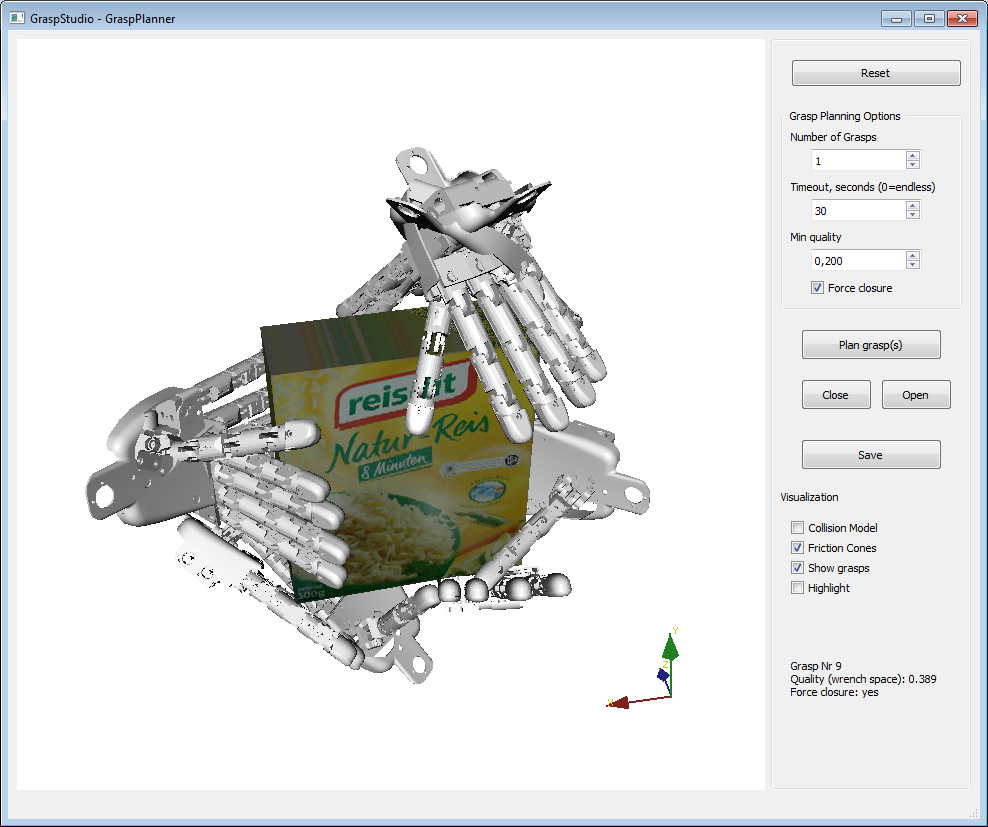
\includegraphics[width=\textwidth]{GraspPlanner}
\subsection{Plan a Grasp}
Grasps can now be planned by calling the plan method of the grasp planner object. Depending on the parameters specified on construction, the grasp planner tries to create the specified number of grasps while respecting the timeout in milliseconds. 
\begin{lstlisting}
// Search one grasp with a timeout of 1000 milliseconds
int graspsPlanned = planner->plan(1,1000);

// retrieve the pose of the grasp
if (graspsPlanned==1)
{
    // mGrasp is the pose of the grasp applied to the global object pose, resulting in the global TCP pose which is related to the grasp
    Eigen::Matrix4f mGrasp = grasps->getGrasp(0)->getTcpPoseGlobal(object->getGlobalPose());
    // now the eef can be set to a position so that it's TCP is at mPose 
    eefCloned->setGlobalPoseForRobotNode(eefCloned->getEndEffector("Left Hand")->getTcp(),mGrasp);
}


// the last computed quality can be retrieved with
float qual = qualityMeasure->getGraspQuality();
bool isFC = qualityMeasure->isGraspForceClosure();


// The contacts information can be retrieved, by closing the end effector
// Additionally the visualization of eefCloned will show the closed fingers
std::vector< VirtualRobot::EndEffector::ContactInfo > contacts = eefCloned->getEndEffector("Left Hand")->closeActors(object);
\end{lstlisting}
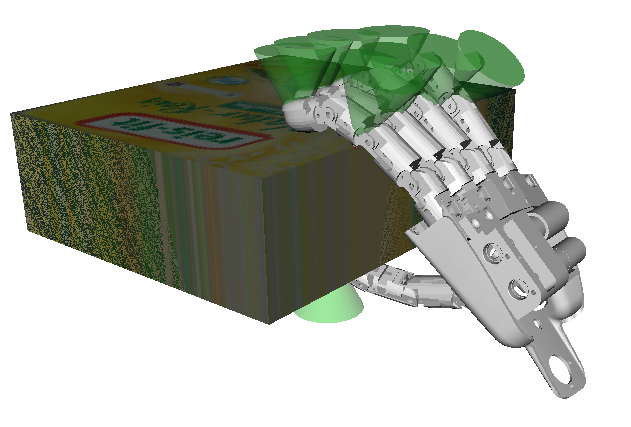
\includegraphics[width=\textwidth]{GraspPlanner1}
\subsection{Store a Set of Grasps}
Grasps can be easily managed by ManipulationObjects, as shown in the following example. A new object is created and cloned instances of the visualization and the collision model are passed to the constructor. Then the set of planned grasps is added and the object is stored to an XML file. The XML file will contain the filename of the visualization model and all grasping information.
\begin{lstlisting}
// create a new object, pass cloned visualizations and collision models to it.
VirtualRobot::ManipulationObjectPtr newObject(new VirtualRobot::ManipulationObject(object->getName(),object->getVisualization()->clone(),object->getCollisionModel()->clone()));

// append the set of planned grasps
newObject->addGraspSet(grasps);

// save to XML file
try
{
    ObjectIO::saveManipulationObject(newObject, "ObjectWithGraspSet.xml");
}
catch (VirtualRobotException &e)
{
    cout << " ERROR while saving object" << endl;
    cout << e.what();
}
\end{lstlisting}
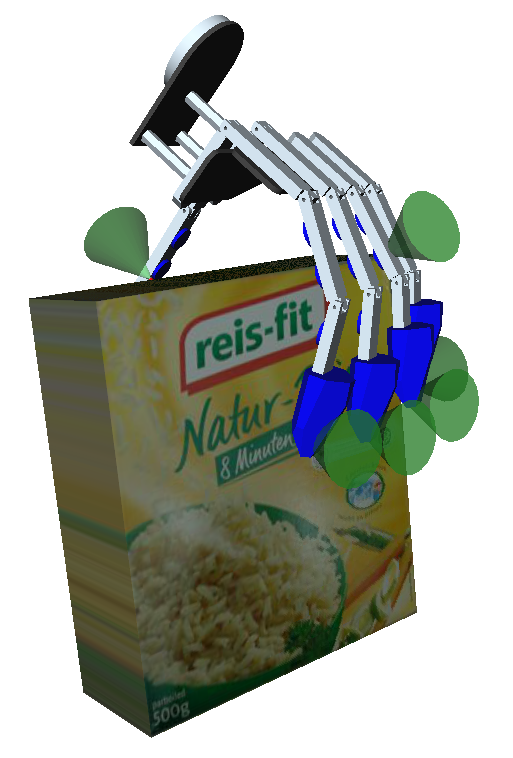
\includegraphics[width=\textwidth]{Grasp1}
\end{document}